\section{main.tex: 大元となり、論文構成を記述}
main.tex には、論文の章立ておよび章を構成するファイルの読み込みを設定する。

main.texファイル内の等外部分で論文構成を決定する。
一つの tex ファイルで論文を書ききることも可能だが、論文の構成や見通しが悪くなるために、このスタイルパッケージでは、main.tex ファイルから複数のtexファイルを読み込むようにしている。
「論文要旨」「謝辞」「論文の各章」「付録」などが、読み込まれるファイルである。

\subsection{論文要旨の読み込み}
まず、論文要旨は以下の形で定義されている。
\begin{breakbox}
{\small
\begin{verbatim}
\chapter*{論文要旨}
\addcontentsline{toc}{chapter}{論文要旨}
近年スマートフォンとオンライン音楽配信サービスの発達により,人々は膨大な数の楽曲を手軽に聴けるようになった.
人々がその膨大な楽曲の中から自分の嗜好にあった楽曲を見つけ出すことは困難であるため,楽曲推薦サービスの需要が高まっている.

楽曲推薦サービスの中でも人間の気分や状況に基づいて楽曲を推薦するサービスをコンテキストアウェアシステムと呼ぶ.
そのシステムの中でも日本語歌詞から人間が感じる印象を推定し,ユーザの気分に合わせて楽曲を推薦する研究は未だ発展途上であった.

本研究ではPLSAによって歌詞中に出現する単語を分析することで,4クラスの潜在的トピックにクラスタリングする.そして得られたモデルパラメータをMAP推定することで,潜在的トピックを喜怒哀楽の4つの印象に制限し,歌詞中に出現する単語から感じとれる印象を推定する.
印象は感性平面上にプロットすることで表現する.歌詞をフレーズごとに分割して,フレーズに登場する単語の印象を合計して正規化することでフレーズの印象とする.
フレーズの印象を合計して正規化することで歌詞全体の印象とする.

歌詞とフレーズに対して推定された印象が妥当であるか有効性を示すために実験をおこなった.
その結果喜の印象推定は妥当であることが確認できた.しかし,その他の印象における推定結果は妥当であるとは言えなかった.
喜のクラスだけが印象推定で有効性を示せた理由はMAP推定に用いた事前知識の数が十分にあったことが一番大きな要因として考えられる.
事前知識の数が少ないとMAP推定する際に無情報事前分布を与えるため,MAP推定前の潜在トピックに属するモデルパラメータと変わらない.
そのためうまく印象を推定できなかったと考慮する.
したがって事前知識を十分確保できた場合,本論で設計した印象推定手法が有効であると期待される.
% abstract.texの中は \chapterなど書かずに単なるテキストを入力する
\end{verbatim}
}
\end{breakbox}
具体的には、\verb+近年スマートフォンとオンライン音楽配信サービスの発達により,人々は膨大な数の楽曲を手軽に聴けるようになった.
人々がその膨大な楽曲の中から自分の嗜好にあった楽曲を見つけ出すことは困難であるため,楽曲推薦サービスの需要が高まっている.

楽曲推薦サービスの中でも人間の気分や状況に基づいて楽曲を推薦するサービスをコンテキストアウェアシステムと呼ぶ.
そのシステムの中でも日本語歌詞から人間が感じる印象を推定し,ユーザの気分に合わせて楽曲を推薦する研究は未だ発展途上であった.

本研究ではPLSAによって歌詞中に出現する単語を分析することで,4クラスの潜在的トピックにクラスタリングする.そして得られたモデルパラメータをMAP推定することで,潜在的トピックを喜怒哀楽の4つの印象に制限し,歌詞中に出現する単語から感じとれる印象を推定する.
印象は感性平面上にプロットすることで表現する.歌詞をフレーズごとに分割して,フレーズに登場する単語の印象を合計して正規化することでフレーズの印象とする.
フレーズの印象を合計して正規化することで歌詞全体の印象とする.

歌詞とフレーズに対して推定された印象が妥当であるか有効性を示すために実験をおこなった.
その結果喜の印象推定は妥当であることが確認できた.しかし,その他の印象における推定結果は妥当であるとは言えなかった.
喜のクラスだけが印象推定で有効性を示せた理由はMAP推定に用いた事前知識の数が十分にあったことが一番大きな要因として考えられる.
事前知識の数が少ないとMAP推定する際に無情報事前分布を与えるため,MAP推定前の潜在トピックに属するモデルパラメータと変わらない.
そのためうまく印象を推定できなかったと考慮する.
したがって事前知識を十分確保できた場合,本論で設計した印象推定手法が有効であると期待される.+となっている部分で、abstract.texファイルを読み込んでいる。
コメントにも書いてあるように、abstract.tex 内には, \verb+\chapter+命令を入れない。

\subsection{謝辞の読み込み}
次に謝辞は以下の様に定義されている。
\begin{breakbox}
{\small
\begin{verbatim}
\chapter*{謝辞}
\addcontentsline{toc}{chapter}{謝辞}
本研究を進めるにあたり,多くの方々にご指導ご鞭撻を賜りました.
指導教員の宮治裕教授からは多大なご指導を賜り,時には過去文献をひも解くヒントなどもご教示いただき感謝の念に堪えません.ありがとうございました.
調査の実施にあたり,宮治研究室の皆さまと同大学の同期には実験参加者を務めて下さり,貴重なデータ収集にご協力いただいたことを感謝いたします.
最後に,本研究ならびに学業全般にわたって経済的・心身的に支援してくださる家族に深く感謝し,お礼を申し上げます.
% thanks.texの中は \chapterなど書かずに単なるテキストを入力する
\end{verbatim}
}
\end{breakbox}
論文要旨と同様に thanks.tex ファイルに \verb+\chapter+命令を入れずに記述する。

\subsection{目次の設定}
次に目次が定義されている。
\begin{breakbox}
{\small
%footnotesize
\begin{verbatim}
%%% 目次
\tableofcontents
\end{verbatim}
}
\end{breakbox}
特に気にせずとも上記命令のままで、目次が自動生成される。

\subsection{各章の読み込み}
ここから各章の記載である。
本パッケージでは、サンプルとして1章〜3章を読み込むようにしている。
具体的には \verb+\include+ 命令で chap1.tex chap2.tex chap3.tex chap4.tex chap5.tex が読み込まれている。
これらのファイル名は、適宜変更して構わない。
また、6章以降の部分はコメントアウトしているが、各自で適宜変更して欲しい。
\begin{breakbox}
{\small
%footnotesize
\begin{verbatim}
\documentclass[a4paper,11pt,oneside,openany]{jsbook}
\usepackage{myjlabthesisstyle}
\daigaku{青山学院大学}
\gakubu{社会情報学部}
\gakka{社会情報学科}
\syubetsu{卒業論文}
\labname{宮治研究室}
\chiefexaminer{宮治~~裕~~教授}

%%%%%%%%%%%%%%%%%%%%%%%%%%%%%%%%%%%%%%%
% ここから先「ここまで個人設定」の範囲に
% 各自の固有の情報を記入して下さい
%%%%%%%%%%%%%%%%%%%%%%%%%%%%%%%%%%%%%%%
\nendo{2021年度}
\teisyutsu{2022年~~1月}
\snum{18118047}
\jname{黒川~~皇輝}
\thesistitle{PLSAとMAP推定を用いた日本語歌詞の印象推定手法の評価} %タイトルを記入
%\thesissubtitle{\LaTeX の利用} %サブタイトルを記入 ない場合はコメントアウト
%\SUBTtrue %サブタイトル有りの場合 ない場合は,コメントアウト
\SUBTfalse %サブタイトル無しの場合 有る場合は,コメントアウト
%%%%%%%%%% ここまで個人設定 %%%%%%%%%%%%%%
\begin{document}

\chapter{はじめに}
本論文では日本語歌詞から得られる印象を推定する手法の設計と実装をし,手法の効果について記述する.
本章では本研究をおこなう背景となった事柄そして研究目的を記述した後,次章以降の本論文の構成についてその概略を述べる.

\section{背景}
近年Amazon Music,Spotifyといった音楽配信サービスとスマートフォンなどのモバイル端末の普及により,人々は膨大な楽曲を手軽に聴くことができるようになった.それに伴い音楽配信サービスのユーザは増加傾向にある[1].
膨大な楽曲の中からユーザが自身の嗜好に合う楽曲を見つけるのは困難であるため,楽曲を推薦するシステムが研究トピックとして着目されている.

音楽推薦システムの中でもユーザの気分や状況に合う楽曲を推薦するシステムをコンテキストアウェア楽曲推薦システムと呼ぶ.コンテキストとは次のように定義されている.
「エンティティの状況を特徴化するのに用いられるあらゆる情報.エンティティとは,ユーザとアプリケーションとのインタラクションに関連する人や場所,オブジェクトを指し,それにはユーザ自身とアプリケーション自体も含まれる」(奥,2019,pp.300\verb+~+308).
コンテキストは大まかにユーザコンテキスト,環境コンテキスト,マルチメディアコンテキストの3つに分類される.ユーザコンテキストはユーザの気分や生体情報である.環境コンテキストは位置情報や時間,天気などのユーザを取り巻く環境情報である.
マルチメディアコンテキストはテキストや映像,画像などの音楽以外のメディアからユーザが得る感性情報である.マルチメディアコンテキストの分野において,日本語歌詞からユーザが受ける印象を推定する手法は研究されているが未だ発展途上である.
\section{研究目的}
本研究の目的は日本語歌詞のテキスト情報をrussellのArousal-Valence平面[2](以下AV平面)上で表現することで,ユーザが感じる歌詞の印象を推定する.
印象推定手法は西川ら(2011)[3]が設計した楽曲印象推定手法を参考に,日本語歌詞から読み取れる印象を推定する手法の設計と評価をおこなう.

\section{論文構成}
2章では関連研究について述べる.
3章では日本語の歌詞の印象推定手法について述べる.
4章では印象推定手法の有効性を確かめるために行なった実験について述べる.
5章では本研究についてのまとめと考察,今後の課題について述べる.

%
\end{document}
 % 1章
\documentclass[a4paper,11pt,oneside,openany]{jsbook}
\usepackage{myjlabthesisstyle}
\daigaku{青山学院大学}
\gakubu{社会情報学部}
\gakka{社会情報学科}
\syubetsu{卒業論文}
\labname{宮治研究室}
\chiefexaminer{宮治~~裕~~教授}

%%%%%%%%%%%%%%%%%%%%%%%%%%%%%%%%%%%%%%%
% ここから先「ここまで個人設定」の範囲に
% 各自の固有の情報を記入して下さい
%%%%%%%%%%%%%%%%%%%%%%%%%%%%%%%%%%%%%%%
\nendo{2021年度}
\teisyutsu{2022年~~1月}
\snum{18118047}
\jname{黒川~~皇輝}
\thesistitle{PLSAとMAP推定を用いた日本語歌詞の印象推定手法の評価} %タイトルを記入
%\thesissubtitle{\LaTeX の利用} %サブタイトルを記入 ない場合はコメントアウト
%\SUBTtrue %サブタイトル有りの場合 ない場合は,コメントアウト
\SUBTfalse %サブタイトル無しの場合 有る場合は,コメントアウト
%%%%%%%%%% ここまで個人設定 %%%%%%%%%%%%%%
\begin{document}

\chapter{宮治研用 \LaTeX スタイルパッケージの使い方}
Microsoft Word やその他のワープロソフトを利用して論文を書いても構わない。
しかしながら宮治研究室では、最終的には \LaTeX によってフォーマットを整えし、PDF化された論文を提出する。

本章では、 \LaTeX で論文を書く際の各種設定などを宮治研究室用に調整したスタイルファイルの利用方法について記述する。

\section{\LaTeX を利用する理由}
\LaTeX を利用するメリットは、デメリットとなる点を考慮しても、非常に大きいと断言できる。
したがって、このデメリットをすこしでも緩和することによって、その利用

が、解消することを目標として、宮治研用の \LaTeX スタイルパッケージを作成し、本文書と共に配布する。


\subsection{\LaTeX を利用するメリット/デメリット}

\LaTeX を利用する際には、HTMLの様なマークアップを文章中に記述する。

適切なマークアップさえすれば、その構造に応じて書式を整形して出力することができる。
また、論文などの文章を書く際の煩雑な手間を、大幅に削減することができる。
その例を一部列挙する。
\begin{itemize}
\item 章や節などの見出しの書式設定は、自動
\item 目次ページ番号、参考文献番号の付加や引用表示、図表や数式の番号割り振りや引用表示が自動
\item 数式がきれいに表現できる
\end{itemize}

その一方で以下の欠点も存在している\cite{test}。
\begin{itemize}
\item \LaTeX が使えるようにソフトウェアを導入しなければならない
\item 最低限のマークアップを憶えなければならない
\item マークアップ以外の命令も憶えなければならない
\end{itemize}


\subsection{デメリットを解決する = 本パッケージの利用}
デメリットを解決するために、宮治研用のスタイルパッケージを整え、本文書を作成した。

\begin{itemize}
\item 「最低限のマークアップ」本文書のサンプルを参考にマネをすれば、完璧に憶える必要はない
\item 「マークアップ以外の命令」自動実行するバッチファイルを準備したため、これを実行するだけで良い
\end{itemize}

よって、\LaTeX の環境を自分のパソコンに整えさえすれば、比較的容易に論文作成ができるであろう。

Macintosh への \LaTeX のインストールは、奥村他有志による TeX Wiki の 「MacTeX のインストール」\cite{mactex} を参考にすると良いだろう。
また、Windows へのインストールは、奥村他有志による TeX Wiki の 「W32Tex」\cite{w32tex} を参考にすると良いだろう。

また、環境構築が困難なもののために以下の二つを用意した。
\begin{itemize}
\item インストールが困難な者に対応するために、Docker環境を準備した
\item Docker環境におけるバッチファイルを準備した
\end{itemize}

したがって、論文を書いたファイルさえあれば、環境構築などに煩わされることなく、\LaTeX による組版が可能となる。
\section{物体の色や表情情報を利用した画像の印象にあった音楽推薦手法の提案}
追木ら(2018)[6]は印象をAV平面上で表現した.英語の歌詞をWord2Vecを用いてArousal-Valence値が既知である印象語と類似度を計算した.Arousal-Valence値が既知である印象語はGeorgios(2013)[7]らが公開されしたものを使用している.
歌詞ともっとも類似度が高い印象語の重みを1として正規化し,各印象の重みつけを行う.各印象語間の角度によるクラスタリング手法であるspherical-kemeans[8]を用いてクラスタリングを行った.クラスタ数は4つであり,AV平面の各象限である.
しかしこの実験では人が認識した印象とシステムが推定した印象の一致率は低かった.
\section{settings.tex: 論文の設定情報を記述}
settings.tex には、各自の個人情報や論文のタイトルなどを設定する。

\subsection{各自の情報設定}
各自の情報を設定する際には、サブタイトルの有り/無しで設定事項が異なることに注意をする必要がある。
それぞれの方法について以下に記述する。
また、これらの作業が終わった時点で、本配布スタイルパッケージの動作確認をすることをおすすめする。

\subsubsection{サブタイトル有りの場合}
配布したファイルは、サブタイトルがある場合のサンプルになっている。
各自の 年度、提出年月、学籍番号、氏名、タイトル、サブタイトルを所定の命令内に記入する。
\begin{breakbox}
{\small
%footnotesize
\begin{verbatim}
\nendo{2013年度}
\teisyutsu{2014年~~1月}
\snum{15387019}
\jname{宮治 裕}
\thesistitle{宮治研における論文作成について} %タイトルを記入
\thesissubtitle{\LaTeX の利用} %サブタイトルを記入 ない場合はコメントアウト
\SUBTtrue %サブタイトル有りの場合 ない場合は、コメントアウト
%\SUBTfalse %サブタイトル無しの場合 有る場合は、コメントアウト
\end{verbatim}
}
\end{breakbox}

\subsubsection{サブタイトル無しの場合}
サブタイトル有りの場合と比較して2箇所の変更が必要である。
サブタイトルを記入する命令の先頭部分に \% 記号を入れ、コメントアウト状態にする。

\begin{breakbox}
{\small
\begin{verbatim}
%\thesissubtitle{\LaTeX の利用} %サブタイトルを記入 無い場合は、コメントアウト
\end{verbatim}
}
\end{breakbox}
もう一つは、その直下の2行
\begin{breakbox}
{\small
\begin{verbatim}
\SUBTtrue %サブタイトル有りの場合 無い場合は、コメントアウト
%\SUBTfalse %サブタイトル無しの場合 有る場合は、コメントアウト
\end{verbatim}
}
\end{breakbox}
以下の様に変更する。
\begin{breakbox}
{\small
\begin{verbatim}
%\SUBTtrue %サブタイトル有りの場合 無い場合は、コメントアウト
\SUBTfalse %サブタイトル無しの場合 有る場合は、コメントアウト
\end{verbatim}
}
\end{breakbox}

以上の設定で、表紙と各ページのヘッダ・フッタの情報が自動的に設定され、書式が整えられる。
\begin{boxnote}
\LaTeX では 「\verb+%+」はコメントを意味し、この記号から改行コードまでをコメントアウト状態として処理する。
\end{boxnote}
であることに注意すること。

\subsection{スタイルパッケージの動作確認}
サブタイトルの有り/無しに応じて適切に設定ができた段階で、一度各自の環境下でスタイルパッケージが正常動作することを確認して欲しい。
正常動作した場合には、本ファイルとほぼ同様の中身で、表紙と各ページのヘッダとフッタが各自の設定した情報が記載されたPDFファイルが出来上がるはずである。

まず、Macintoshの場合について記す。
各自のホームディレクトリ中のDropboxフォルダ内に、本スタイルパッケージが展開されている場合を前提として記述する。
\begin{enumerate}
\item まず、ターミナルを開く
\item 以下のコマンドを入力し、スタイルパッケージのあるフォルダに移動
\footnote{ここで \verb+$+記号は、コマンドプロンプトを表すため、入力しないように。}
\begin{screen}
{\small
\begin{verbatim}
 $ cd ~/Dropbox/Thesis
\end{verbatim}
}
\end{screen}

\item そこで、バッチファイル \verb+mklatex.bat+ を実行
\begin{screen}
{\small
\begin{verbatim}
 $ ./mklatex.bat
\end{verbatim}
}
\end{screen}

\item main.pdfファイルが作成され、プレビュー画面が自動で表示される
\item[\textbf{注}] mklatex.bat が実行できないというようなエラーが出た場合には、最初の一回だけ(次回から不要)以下の命令を入力する
\begin{screen}
{\small
\begin{verbatim}
 $ chmod 755 ./mklatex.bat
\end{verbatim}
}
\end{screen}
\end{enumerate}

正常動作しなかった場合には、出来上がった main.log ファイルを宮治に送付して欲しい。

Windowsの場合には、コマンドプロンプトを開き、目的のフォルダに移動し、バッチファイル(winmklatex.bat)を起動する。
\begin{screen}
{\small
\begin{verbatim}
 $ cd c:\My Documents\Dropbox\Thesis
 $ winmklatex.bat
\end{verbatim}
}
\end{screen}
main.pdfファイルができるので、エクスプローラからファイルをダブルクリックしてAcrobat Reader にて確認して欲しい。


\section{main.tex: 大元となり、論文構成を記述}
main.tex には、論文の章立ておよび章を構成するファイルの読み込みを設定する。

main.texファイル内の等外部分で論文構成を決定する。
一つの tex ファイルで論文を書ききることも可能だが、論文の構成や見通しが悪くなるために、このスタイルパッケージでは、main.tex ファイルから複数のtexファイルを読み込むようにしている。
「論文要旨」「謝辞」「論文の各章」「付録」などが、読み込まれるファイルである。

\subsection{論文要旨の読み込み}
まず、論文要旨は以下の形で定義されている。
\begin{breakbox}
{\small
\begin{verbatim}
\chapter*{論文要旨}
\addcontentsline{toc}{chapter}{論文要旨}
近年スマートフォンとオンライン音楽配信サービスの発達により,人々は膨大な数の楽曲を手軽に聴けるようになった.
人々がその膨大な楽曲の中から自分の嗜好にあった楽曲を見つけ出すことは困難であるため,楽曲推薦サービスの需要が高まっている.

楽曲推薦サービスの中でも人間の気分や状況に基づいて楽曲を推薦するサービスをコンテキストアウェアシステムと呼ぶ.
そのシステムの中でも日本語歌詞から人間が感じる印象を推定し,ユーザの気分に合わせて楽曲を推薦する研究は未だ発展途上であった.

本研究ではPLSAによって歌詞中に出現する単語を分析することで,4クラスの潜在的トピックにクラスタリングする.そして得られたモデルパラメータをMAP推定することで,潜在的トピックを喜怒哀楽の4つの印象に制限し,歌詞中に出現する単語から感じとれる印象を推定する.
印象は感性平面上にプロットすることで表現する.歌詞をフレーズごとに分割して,フレーズに登場する単語の印象を合計して正規化することでフレーズの印象とする.
フレーズの印象を合計して正規化することで歌詞全体の印象とする.

歌詞とフレーズに対して推定された印象が妥当であるか有効性を示すために実験をおこなった.
その結果喜の印象推定は妥当であることが確認できた.しかし,その他の印象における推定結果は妥当であるとは言えなかった.
喜のクラスだけが印象推定で有効性を示せた理由はMAP推定に用いた事前知識の数が十分にあったことが一番大きな要因として考えられる.
事前知識の数が少ないとMAP推定する際に無情報事前分布を与えるため,MAP推定前の潜在トピックに属するモデルパラメータと変わらない.
そのためうまく印象を推定できなかったと考慮する.
したがって事前知識を十分確保できた場合,本論で設計した印象推定手法が有効であると期待される.
% abstract.texの中は \chapterなど書かずに単なるテキストを入力する
\end{verbatim}
}
\end{breakbox}
具体的には、\verb+近年スマートフォンとオンライン音楽配信サービスの発達により,人々は膨大な数の楽曲を手軽に聴けるようになった.
人々がその膨大な楽曲の中から自分の嗜好にあった楽曲を見つけ出すことは困難であるため,楽曲推薦サービスの需要が高まっている.

楽曲推薦サービスの中でも人間の気分や状況に基づいて楽曲を推薦するサービスをコンテキストアウェアシステムと呼ぶ.
そのシステムの中でも日本語歌詞から人間が感じる印象を推定し,ユーザの気分に合わせて楽曲を推薦する研究は未だ発展途上であった.

本研究ではPLSAによって歌詞中に出現する単語を分析することで,4クラスの潜在的トピックにクラスタリングする.そして得られたモデルパラメータをMAP推定することで,潜在的トピックを喜怒哀楽の4つの印象に制限し,歌詞中に出現する単語から感じとれる印象を推定する.
印象は感性平面上にプロットすることで表現する.歌詞をフレーズごとに分割して,フレーズに登場する単語の印象を合計して正規化することでフレーズの印象とする.
フレーズの印象を合計して正規化することで歌詞全体の印象とする.

歌詞とフレーズに対して推定された印象が妥当であるか有効性を示すために実験をおこなった.
その結果喜の印象推定は妥当であることが確認できた.しかし,その他の印象における推定結果は妥当であるとは言えなかった.
喜のクラスだけが印象推定で有効性を示せた理由はMAP推定に用いた事前知識の数が十分にあったことが一番大きな要因として考えられる.
事前知識の数が少ないとMAP推定する際に無情報事前分布を与えるため,MAP推定前の潜在トピックに属するモデルパラメータと変わらない.
そのためうまく印象を推定できなかったと考慮する.
したがって事前知識を十分確保できた場合,本論で設計した印象推定手法が有効であると期待される.+となっている部分で、abstract.texファイルを読み込んでいる。
コメントにも書いてあるように、abstract.tex 内には, \verb+\chapter+命令を入れない。

\subsection{謝辞の読み込み}
次に謝辞は以下の様に定義されている。
\begin{breakbox}
{\small
\begin{verbatim}
\chapter*{謝辞}
\addcontentsline{toc}{chapter}{謝辞}
本研究を進めるにあたり,多くの方々にご指導ご鞭撻を賜りました.
指導教員の宮治裕教授からは多大なご指導を賜り,時には過去文献をひも解くヒントなどもご教示いただき感謝の念に堪えません.ありがとうございました.
調査の実施にあたり,宮治研究室の皆さまと同大学の同期には実験参加者を務めて下さり,貴重なデータ収集にご協力いただいたことを感謝いたします.
最後に,本研究ならびに学業全般にわたって経済的・心身的に支援してくださる家族に深く感謝し,お礼を申し上げます.
% thanks.texの中は \chapterなど書かずに単なるテキストを入力する
\end{verbatim}
}
\end{breakbox}
論文要旨と同様に thanks.tex ファイルに \verb+\chapter+命令を入れずに記述する。

\subsection{目次の設定}
次に目次が定義されている。
\begin{breakbox}
{\small
%footnotesize
\begin{verbatim}
%%% 目次
\tableofcontents
\end{verbatim}
}
\end{breakbox}
特に気にせずとも上記命令のままで、目次が自動生成される。

\subsection{各章の読み込み}
ここから各章の記載である。
本パッケージでは、サンプルとして1章〜3章を読み込むようにしている。
具体的には \verb+\include+ 命令で chap1.tex chap2.tex chap3.tex chap4.tex chap5.tex が読み込まれている。
これらのファイル名は、適宜変更して構わない。
また、6章以降の部分はコメントアウトしているが、各自で適宜変更して欲しい。
\begin{breakbox}
{\small
%footnotesize
\begin{verbatim}
\documentclass[a4paper,11pt,oneside,openany]{jsbook}
\usepackage{myjlabthesisstyle}
\input{settings}
\begin{document}

\chapter{はじめに}
本論文では日本語歌詞から得られる印象を推定する手法の設計と実装をし,手法の効果について記述する.
本章では本研究をおこなう背景となった事柄そして研究目的を記述した後,次章以降の本論文の構成についてその概略を述べる.

\section{背景}
近年Amazon Music,Spotifyといった音楽配信サービスとスマートフォンなどのモバイル端末の普及により,人々は膨大な楽曲を手軽に聴くことができるようになった.それに伴い音楽配信サービスのユーザは増加傾向にある[1].
膨大な楽曲の中からユーザが自身の嗜好に合う楽曲を見つけるのは困難であるため,楽曲を推薦するシステムが研究トピックとして着目されている.

音楽推薦システムの中でもユーザの気分や状況に合う楽曲を推薦するシステムをコンテキストアウェア楽曲推薦システムと呼ぶ.コンテキストとは次のように定義されている.
「エンティティの状況を特徴化するのに用いられるあらゆる情報.エンティティとは,ユーザとアプリケーションとのインタラクションに関連する人や場所,オブジェクトを指し,それにはユーザ自身とアプリケーション自体も含まれる」(奥,2019,pp.300\verb+~+308).
コンテキストは大まかにユーザコンテキスト,環境コンテキスト,マルチメディアコンテキストの3つに分類される.ユーザコンテキストはユーザの気分や生体情報である.環境コンテキストは位置情報や時間,天気などのユーザを取り巻く環境情報である.
マルチメディアコンテキストはテキストや映像,画像などの音楽以外のメディアからユーザが得る感性情報である.マルチメディアコンテキストの分野において,日本語歌詞からユーザが受ける印象を推定する手法は研究されているが未だ発展途上である.
\section{研究目的}
本研究の目的は日本語歌詞のテキスト情報をrussellのArousal-Valence平面[2](以下AV平面)上で表現することで,ユーザが感じる歌詞の印象を推定する.
印象推定手法は西川ら(2011)[3]が設計した楽曲印象推定手法を参考に,日本語歌詞から読み取れる印象を推定する手法の設計と評価をおこなう.

\section{論文構成}
2章では関連研究について述べる.
3章では日本語の歌詞の印象推定手法について述べる.
4章では印象推定手法の有効性を確かめるために行なった実験について述べる.
5章では本研究についてのまとめと考察,今後の課題について述べる.

%
\end{document}
 % 1章
\documentclass[a4paper,11pt,oneside,openany]{jsbook}
\usepackage{myjlabthesisstyle}
\input{settings}
\begin{document}

\chapter{宮治研用 \LaTeX スタイルパッケージの使い方}
Microsoft Word やその他のワープロソフトを利用して論文を書いても構わない。
しかしながら宮治研究室では、最終的には \LaTeX によってフォーマットを整えし、PDF化された論文を提出する。

本章では、 \LaTeX で論文を書く際の各種設定などを宮治研究室用に調整したスタイルファイルの利用方法について記述する。

\input{sec21}
\input{sec22}
\input{sec23}
\input{sec24}
%
\end{document} % 2章
\documentclass[a4paper,11pt,oneside,openany]{jsbook}
\usepackage{myjlabthesisstyle}
\input{settings}
\begin{document}

\chapter{歌詞の印象推定}
本研究で行った歌詞の印象推定法について説明する.最初に研究で用いた分析手法について述べたのちに,分析手法を活用した歌詞の印象推定手法について述べる.その後,分析結果を記述する.
\input{sec31}
\input{sec32}
\input{sec33}
%
\end{document} % 3章
\documentclass[a4paper,11pt,oneside,openany]{jsbook}
\usepackage{myjlabthesisstyle}
\input{settings}
\begin{document}

\chapter{Visual Studio Codeで編集する人へ}
Visual Studio Codeを使って \LaTeX 論文を作成する人が増えているため、それに合わせた修正を各所でおこなっている。
以下の設定や、注意事項を参照してほしい。

\section{コンパイルのための設定}
\LaTeX をコンパイルする際には、目次や参照、参考文献などを組み込むための処理などを複数回実行する必要がある。
これを自動で判断して実行するための設定ファイルが \verb+.latexmkrc+である。
本スタイルファイルパッケージでは、以下の設定をしている。
\begin{screen}
{\small
\begin{verbatim}
#!/usr/bin/env perl
$pdf_mode = 3;
$latex = 'platex -halt-on-error';
$bibtex = 'pbibtex';
$dvipdf = 'dvipdfmx %O -o %D %S';
\end{verbatim}    
}
\end{screen}

なお、一部の行を割愛して表示している。
詳細は、直接ファイルを確認してほしい。

情報源として、以下の2サイトを記載する。
Macintosh だけでなく、WindowsやLinuxでの利用(特にプレビュー)を含めた設定については、\verb+@popunbom+氏のQiitaの記事「VSCode で LaTeX を書く (2018)」~\cite{popunbom1}が詳しい。
LaTeXをインストールしたり、利用したりする際の情報源である \TeX Wiki にも「Visual Studio Code/LaTeX」~\cite{texwikivscode}なるページがある。

\section{LaTeX Workshop の設定}
VSCodeプラグインであるLaTeX Workshopの設定は、以下の様にしている。
なお、必ずしも同じ設定にする必要はない。
\begin{screen}
{\footnotesize
\begin{verbatim}
"latex-workshop.latex.tools": [
  {
    "name": "Latexmk (pLaTeX)",
    "command": "latexmk",
    "args": [
      "-f",
      "-gg",
      "-pv",
      "-latex='platex'",
      "-synctex=1",
      "-interaction=nonstopmode",
      "-file-line-error",
      "%DOC%"
    ]
  },
],
\end{verbatim}
}
\end{screen}
\begin{screen}
    {\footnotesize
    \begin{verbatim}
"latex-workshop.latex.recipes": [
  {
    "name": "pLaTeX",
    "tools": [
      "Latexmk (pLaTeX)"
    ]
  },
],
\end{verbatim}
}
\end{screen}
\begin{screen}
{\footnotesize
\begin{verbatim}
"latex-workshop.latex.magic.args": [
  "-f",
  "-gg",
  "-pv",
  "-synctex=1",
  "-interaction=nonstopmode",
  "-file-line-error",
  "%DOC%"
],
\end{verbatim}
}
\end{screen}
\begin{screen}
{\footnotesize
\begin{verbatim}
"latex-workshop.view.pdf.viewer":"tab",
"latex-workshop.latex.autoBuild.run": "never",
"latex-workshop.view.pdf.refviewer":"tabOrBrowser",
"latex-workshop.latex.autoClean.run":"onBuilt",
\end{verbatim}
}
\end{screen}

\section{分割(子ファイル)コンパイル}
通常の \LaTeX のファイルの場合に親ファイルに記述する文書開始や終了/スタイルファイルの読み込みを子ファイル側に書き込むことによって、それぞれのファイルごとにコンパイルができる。

\begin{screen}
{\footnotesize
\begin{verbatim}
\documentclass[a4paper,10pt,twocolumn]{jsarticle}
\usepackage{myjlababsstyle}
\begin{document}
\section{これは読み込まれる子ファイルの例}
ファイル名は sub.tex とします。
\end{document}
\end{verbatim}
}
\end{screen}

これを読み込む親ファイル側では、これらの設定を無視するようにしなければならない。
そのために、\verb+docmute+パッケージを用いている。
親ファイルの例を以下に示す。
\begin{screen}
{\footnotesize
\begin{verbatim}
\documentclass[a4paper,10pt,twocolumn]{jsarticle}
\usepackage{docmute}
\usepackage{myjlababsstyle}
\begin{document}
これは親ファイルの例です。
\input{sub}
\end{document}
\end{verbatim}
}
\end{screen}

また、多くのスタイルファイルを親ファイルと子ファイルで共通して読み込むために、スタイルファイルを \verb+myjlababsstyle.sty+ ファイル内に列挙している。
各自でスタイルファイルを追加する場合には、このファイルに記載すること。

\section{テキスト校正くん}
「テキスト校正くん」パッケージは追加すべきである。
ただし、\LaTeX のファイルは校正してくれないため、\verb+txt+か\verb+md+のファイルを作成し、そこに文章を貼り付けて校正するのが良い。
インストールや設定などが必要ない「テキスト校正くん」を利用することにしたが、昨年まではRedpenと比較して細かい部分の校正は不十分である。
最低限の校正として必ず利用してほしい。
%
\end{document}
 % 4章
\documentclass[a4paper,11pt,oneside,openany]{jsbook}
\usepackage{myjlabthesisstyle}
\input{settings}
\begin{document}

\chapter{おわりに}
本章では本研究のまとめと今後の課題について述べる.
\section{まとめ}
本研究ではコンテキストアウェア楽曲推薦システムの今後の発展のために日本語歌詞の印象推定手法の設計と効果測定をおこなった.
従来の歌詞の印象推定手法は未だ発展途上にあり,詳細に印象推定できる手法は未だ存在しない.そのため西川らの設計した印象推定手法に基づき日本語歌詞の印象推定方法を設計した.
4章で述べた実験結果より設計した印象推定手法は一部の印象において妥当であることが判明した.しかし,全体的には印象を推定することは叶わなかったと言える.
一部の印象を推定できた理由としては事前知識が十分に存在したことが考えられる.
\section{今後の課題}
今後の課題は2点ある.1つ目は事前知識を増やす必要があることである.日本語版ANEW拡張データセットは印象においてデータ数に偏りが認められ,印象推定の結果が妥当であると判断された印象の事前知識は不当であると判断された印象よりも2,000語多く存在した.
したがって推定結果が不当であった印象における事前知識を増やす必要があると考える.
2つ目は歌詞から得られる印象が必ずしも1つではないということを考慮する必要があることである.歌詞全体の印象はフレーズから得られる印象の合計値であると本研究では推測して実験をおこなった.
しかし,歌詞によっては複数の印象を与える歌詞も存在するため,必ずしも1つの印象に推定することは正しいと言えない.そのため,複数の印象を推定するという観点で推定手法を設計し直す必要がある.
\end{document} % 5章
%\include{chap6} % 6章
%\include{chap7} % 7章
\end{verbatim}
}
\end{breakbox}

なお、これらのファイルは通常の\verb+\chapter+など \LaTeX の命令でマークアップしていけば良い。
chapter1.tex や chapter2.tex、chapter3.tex 内を見れば、おおよその方法は理解できるはずである。

\subsection{付録の設定と読み込み}
付録は以下の様になっている。
\begin{breakbox}
{\small
%footnotesize
\begin{verbatim}
%%% 付録 -- 必要なければ以下を2行コメントアウト
\appendix
\documentclass[a4paper,11pt,oneside,openany]{jsbook}
\usepackage{myjlabthesisstyle}
\input{settings}
\begin{document}

\chapter{プログラムの動作方法}
本研究にて用いたプログラムについて解説する。

\section{ファイル構成}
プログラムのフォルダ内は、主に4つのファイルから構成される。

ああああいいいい

ううううええええ

これらを○○に設置し、以下の手順にそって起動する。

\section{起動方法}
まず、ウェブサーバを動かした状態にし、外部クライアント(Webブラウザから)、以下のURLにアクセスする。


\section{表示の見方}
実験に利用するための、実行結果は test.log ファイルに出力されている。

このファイルは4つのカラムからなる CSV形式のファイルである。
第1列には、…

%
\end{document}




%\include{appendixB} %必要に応じて付録の数を増やす
\end{verbatim}
}
\end{breakbox}
サンプルとして 付録A(appendixA.tex)だけ読み込む様にしている。
このファイルも通常の\verb+\chapter+など通常の\LaTeX の命令でマークアップしていけば良い。
また、必要に応じて追加、コメントアウトして構わない。

\subsection{参考文献の設定と読み込み}
最後に参考文献の設定がなされている。
\begin{breakbox}
{\small
%footnotesize
\begin{verbatim}
\bibliographystyle{junsrt}
\bibliography{myrefs}
\end{verbatim}
}
\end{breakbox}
\verb+\bibliography{myrefs}+によって myrefs.bib ファイルが読み込まれている。
このファイルは \BibTeX のフォーマットにて記載されている。
詳細は3章にて記述する。

%
\end{document} % 2章
\documentclass[a4paper,11pt,oneside,openany]{jsbook}
\usepackage{myjlabthesisstyle}
\daigaku{青山学院大学}
\gakubu{社会情報学部}
\gakka{社会情報学科}
\syubetsu{卒業論文}
\labname{宮治研究室}
\chiefexaminer{宮治~~裕~~教授}

%%%%%%%%%%%%%%%%%%%%%%%%%%%%%%%%%%%%%%%
% ここから先「ここまで個人設定」の範囲に
% 各自の固有の情報を記入して下さい
%%%%%%%%%%%%%%%%%%%%%%%%%%%%%%%%%%%%%%%
\nendo{2021年度}
\teisyutsu{2022年~~1月}
\snum{18118047}
\jname{黒川~~皇輝}
\thesistitle{PLSAとMAP推定を用いた日本語歌詞の印象推定手法の評価} %タイトルを記入
%\thesissubtitle{\LaTeX の利用} %サブタイトルを記入 ない場合はコメントアウト
%\SUBTtrue %サブタイトル有りの場合 ない場合は,コメントアウト
\SUBTfalse %サブタイトル無しの場合 有る場合は,コメントアウト
%%%%%%%%%% ここまで個人設定 %%%%%%%%%%%%%%
\begin{document}

\chapter{歌詞の印象推定}
本研究で行った歌詞の印象推定法について説明する.最初に研究で用いた分析手法について述べたのちに,分析手法を活用した歌詞の印象推定手法について述べる.その後,分析結果を記述する.
\section{分析手法}
この節では歌詞印象推定手法で用いた分析手法について紹介する.
\subsection{MAP推定}
MAP推定とは事前知識に基づいて未知のデータを点推定する手法である.
θを尤度,Dを事前知識とすると,ベイズの定理に基づき次の式(3.1)で表せる.
\begin{equation}
\begin{split}
\rm{argmax_{θ}P(θ|D)}&\rm{=argmax_θ\frac{P(D|θ)P(θ)}{P(D)}}\\
&\rm{=argmax_{θ}P(D|θ)P(θ)}
\end{split}
\end{equation}
ここで分母のP(D)は尤度θと関係がないので無視する.P(D\verb+|+θ)は尤度関数,P(θ)は事前分布,P(θ\verb+|+D)は事後分布と呼ぶ.
事前分布P(θ)は複雑な計算を要する.そのため,それを回避するために事前分布の代わりに共役事前分布を用いて推定をする.共役事前分布とは尤度をかけて事後分布を求めるとその関数の形が同じになる事前分布のことである.
事後分布が最大となる尤度θを算出するのがMAP推定である.

本研究ではカテゴリカル分布に基づくMAP推定をする.
したがって事前知識Dはカテゴリカル分布に従うN個の離散値データ$\rm{D=\{d_1,d_2,...d_N\}}$と定義する.
尤度関数はカテゴリカル分布の確立質量関数で表せるので式(3.2)となる.
\begin{equation}
\begin{split}
\rm{P(D|θ)=\prod^N_{n=1}Cat(d_n|θ)}
\end{split}
\end{equation}
カテゴリカル分布の共役事前分布はディリクレ分布であるため事前分布を式(3.3)で表す.ディリクレ分布はハイパーパラメータαが大きくなるにつれて分散が小さくなる特性を持つ.
ハイパーパラメータαは対応する事象dの観測数の初期値を意味する.αを全て1とした場合,ディリクレ分布は一様な無情報事前分布となり,事後分布は尤度関数であるカテゴリカル分布と同じ分布になる.
\begin{equation}
\begin{split}
\rm{P(θ)\propto{Dir(θ;\alpha)}}
\end{split}
\end{equation}
式(3.2)と式(3.3)を式(3.1)に当てはめると事後分布は式(3.4)のように表せる.
\begin{equation}
\begin{split}
\rm{P(θ|D)\propto\{\prod^N_{n=1}Cat(d_n|θ)\}Dir(θ;\alpha)}
\end{split}
\end{equation}
式(3.4)の両辺に対数をとった式(3.5)を示す.ここで$\rm{d_{n,k}}$はK次元ベクトル$\rm{d_n}$のk番目の要素を指し示す.$\mathbb{C}$は不定定数である.
\begin{equation}
\begin{split}
\rm{\log P(θ|D)}&\rm{\propto\sum^N_{n=1}\log Cat(d_n|θ)+\log Dir(θ;\alpha)+\mathbb{C}}\\
&\rm{=\sum^K_{k=1}(\sum^N_{n=1}d_{n,k}+\alpha_{n,k}-1)\log θ_k+\mathbb{C}}
\end{split}
\end{equation}
このまま偏微分しても極値を得ることはできないのでラグランジュの未定乗数法を使用する.ラグランジュ関数は式(3.6)である.
\begin{equation}
\begin{split}
\rm{L=\log P(θ|D)+\lambda(\sum^K_{k=1}θ_k-1)}
\end{split}
\end{equation}
ラグランジュ関数Lを$\rm{θ_k}$で偏微分して0となる極値を求めるとMAP推定値$\rm{{\hat\mu}_{map,k}}$が得られる.
\begin{equation}
\begin{split}
\rm{{\hat\mu}_{map,k}=\frac{\alpha_k-1+θ_k}{1-K+\sum^K_{j=1}\alpha_j}}
\end{split}
\end{equation}
\subsection{PLSA}
PLSA[12]とは次元圧縮手法の一種であり,情報検索の分野で膨大な文書データを分類するために研究された手法である.
PLSAは文書dとその文書中に出現する単語wの間に共通のトピックと呼ぶ潜在意味クラスzが存在することを想定として,潜在意味クラスzを確率的に推定する手法である.
そして,文書dと単語wの共起確率P(d,w)を潜在意味クラスzを用いてモデル化する.zでモデル化したP(d,w)の式を式(3.8)にグラフィカルモデルを図1に示す.
\begin{equation}
\begin{split}
\rm{P(d,w)=\sum_zP(z)P(d|z)P(w|z)}
\end{split}
\end{equation}

\begin{figure}[h]
  \centering
  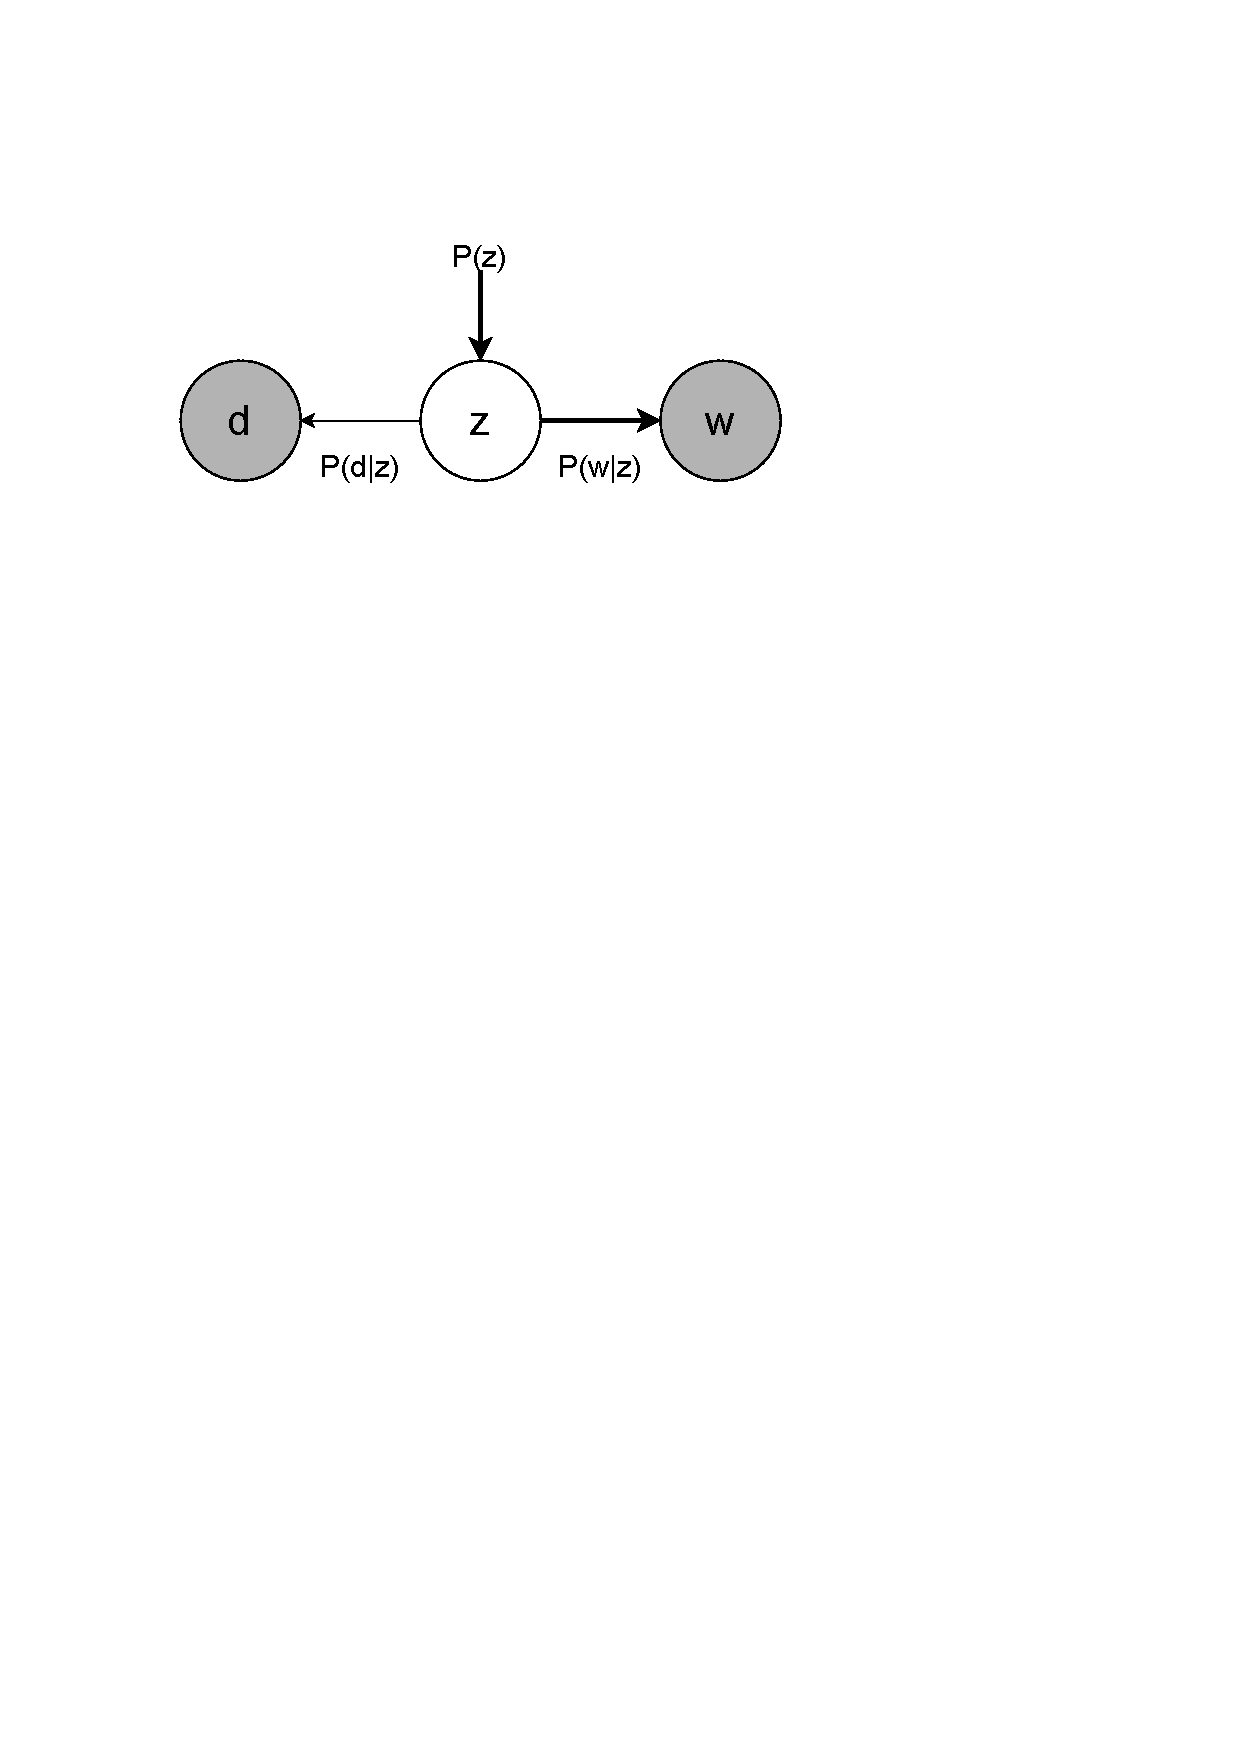
\includegraphics[width=12cm]{PLSA_graphical.pdf}
  \vspace{-1mm}
  \caption{PLSAグラフィカルモデル}
  \label{fig:vkall}
  \vspace{5mm}
\end{figure}
文書dと単語wの同時出現頻度をN(d,w)とすると,対数尤度関数logLは式(3.9)として示せる.
\begin{equation}
\begin{split}
\rm{\log L= \sum_d\sum_wN(d,w)\log(P(d,w))}
\end{split}
\end{equation}
この対数尤度関数logLを最大にする確率変数P(z),P(d\verb+|+z),P(w\verb+|+z)をEMアルゴリズムによって推定する.なお推定する確率変数をモデルパラメータと呼ぶ.EMアルゴリズムとは混合分布モデルのパラメータ推定に利用できる学習アルゴリズムである.
zの確率分布P(z\verb+|+d,w)を予測するE(expectation)ステップと対数尤度関数の最大化をするM(maximization)ステップに計算ステップが分かれている.それぞれのステップで行われる計算の説明を順番に述べる.
式(3.10)はEステップの式である.初期値であるP(z),P(d\verb+|+z),P(w\verb+|+z)は絶対値が1以下のランダムな自然数に決定され,zの確率分布P(z\verb+|+d,w)を予測する.

\begin{equation}
\rm{P(z|d,w)=\frac{P(d|z)P(w|z)P(z)}{\sum_zP(d|z)P(w|z)P(z)}}
\end{equation}
式(3.11)(3.12)(3.13)はMステップの式であり,それぞれの式でモデルパラメータを求めている.

\begin{equation}
\rm{P(d|z)=\frac{\sum_wN(d,w)P(z|d,w)}{\sum_d\sum_wN(d,w)P(z|d,w)}}
\end{equation}

\begin{equation}
\rm{P(w|z)=\frac{\sum_dN(d,w)P(z|d,w)}{\sum_d\sum_wN(d,w)P(z|d,w)}}
\end{equation}

\begin{equation}
\rm{P(z)=\frac{\sum_d\sum_wN(d,w)P(z|d,w)}{\sum_d\sum_w\sum_zN(d,w)P(z|d,w)}}
\end{equation}
求めたモデルパラメータを式(3.2)に当てはめて式(3.3)の対数尤度関数の値を求める.対数尤度関数の値を最大化するまでEステップとMステップを交互に繰り返し,最適なモデルパラメータを求める.

\subsection{日本語版ANEW拡張データセット}
本間らが開発した日本語版ANEWの単語の類義語と同義語をWordNet[14]を用いて探索する.発見した単語に類義語元の単語が持つArousalとValenceの値を与えることで,日本語版ANEWを14,232語に拡張した単語データセットを日本語版ANEW拡張データセットとする.
日本語版ANEW拡張データセットの構成は後述するA+V+平面に5,581語,A+V-平面に2,681語,A-V-平面に3,456語,A-V+平面に2,493語である.
\newpage
\section{歌詞の印象推定手法}
この節では歌詞の印象推定手法について紹介する.

\subsection{印象の定義}
本稿で推定する印象とはRussellのAV平面上で表現する.AV平面は縦軸にArousalを,横軸にValenceを取る2次元平面である.Arousal軸は正の方向に興奮を,負の方向に弛緩を表す.そして,Valence軸は正の方向に快を,負の方向に不快を表す.
AV平面の4象限は大まかに喜怒哀楽の印象を表す.第1象限は喜びや幸福,興奮,驚きといった喜の感情グループを表す.第2印象は怒りや恐れ,嫌悪といった怒の感情グループを表す.第3章限は退屈や悲しみ,
憂鬱といった哀の感情グループを表す.第4象限は満足や穏やか,くつろぎといった楽の感情グループを表す.AV平面に歌詞データをプロットし,データが存在する象限から歌詞データを4つのグループの印象にクラスタリングする.

\subsection{歌詞データの収集}
歌詞データの収集はUta-Net\footnote{https://www.uta-net.com/}から人気のアーティストの曲を6,813曲収集した.本研究では6,813曲から3,000曲を無作為に選んだ.

\subsection{歌詞データの整形}
収集した歌詞データの中に一部英語が入っていたので,英語の歌詞を削除した.そして歌詞データを歌詞のフレーズごとに分解した.形態素解析器MeCabを用いて各フレーズから名詞・形容詞・動詞を抜き出した.歌詞から抜き出した単語の総数は109450語である.

\subsection{歌詞印象推定}
確率的潜在意味解析(PLSA)を利用する.歌詞のフレーズを文書dとし,フレーズ中に出現する単語を単語wと定義してモデルパラメータを推定した.
P(w\verb+|+z)はトピックから単語が観測される確率であるため,この確率の高い単語がトピックを表現する.
歌詞の印象を推定するためには潜在的なトピックzを印象に制限する必要がある.通常のPLSAは文書と単語の共起確率に着目して,潜在的なトピックを推定する手法であるため,必ず潜在的なトピックが印象を表現するとは限らない.
よって,日本語版ANEW拡張データセットを事前知識として使用し,モデルパラメータをMAP推定することで潜在的なトピックにAV平面の各象限を表現する.
具体的に潜在的なトピックzを次の式(3.14)のようにAV平面の各印象として定義する.
\begin{equation}
\rm{z\in\{A+V+,A+V-,A-V-,A-V+\}}
\end{equation}
モデルパラメータP(w\verb+|+z)の対数事前分布を共役事前分布を用いて式(3.15)に定義する.kは出現する単語の集合を表す.
\begin{equation}
\rm{log P(w_k|z)\propto\sum_k\sum_z(\alpha_{w_k,z}-1)\log P(w_k|z)}
\end{equation}
共役事前分布のハイパーパラメータαは日本語版ANEW拡張データセットに含まれる単語で該当の象限に位置する場合のみ原点からの距離を入力する.それ以外の場合無情報事前分布を与える.
ラグランジュの未定乗数法を使用して対数尤度関数と対数事前分布よりMAP推定値を求める
MAP推定値は式(3.16)で表す.NはMAP推定前のP(w\verb+|+z)の和である.
\begin{equation}
\rm{P(w_k|z)_{map}=\frac{\alpha_{w_k,z}-1+p(w_k|z)}{1-K+\sum_k\alpha_{w_k,z}}}
\end{equation}
P(z)とP(d\verb+|+z)の推定には無情報事前分布を与えた.
各印象ごとに単語wが出現する確率P(w\verb+|+z)をMAP推定した.ベイズの定理よりP(z\verb+|+w)は式(3.17)で求められる.
\begin{equation}
\rm{P(z|w_k)=\frac{P(w_k|z)_{map}P(z)}{P(w_k)}}
\end{equation}
P(w)は単語が出現する確率である.ある単語の出現数を全ての単語の出現数で割ると求まる.
各フレーズdのArousalとValenceの値は求めたP(z\verb+|+w)を用いて求めた各単語wのArousalとValenceの値を合計.正規化して求める.式は(3.18,3.19)である.Kはあるフレーズに出現する単語数である.
\begin{equation}
\rm{V=\frac{1}{K} \sum_{k=1}^{K}\left(\left(P\left(\mathrm{~A}+\mathrm{V}+\mid w_{k}\right)+P\left(\mathrm{~A}-\mathrm{V}+\mid w_{k}\right)\right)-\left(P\left(\mathrm{~A}+\mathrm{V}-\mid w_{k}\right)+P\left(\mathrm{~A}-\mathrm{V}-\mid w_{k}\right)\right)\right)}
\end{equation}
\begin{equation}
\rm{A=\frac{1}{K} \sum_{k=1}^{K}\left(\left(P\left(\mathrm{~A}+\mathrm{V}+\mid w_{k}\right)+P\left(\mathrm{~A}+\mathrm{V}-\mid w_{k}\right)\right)-\left(P\left(\mathrm{~A}-\mathrm{V};\mid w_{k}\right)+P\left(\mathrm{~A}-\mathrm{V}-\mid w_{k}\right)\right)\right)}
\end{equation}
以上で歌詞中のフレーズごとに感情価を求める.
\newpage
\section{AV平面にプロット}
この節では歌詞をAV平面上にプロットした結果について記述する.

\subsection{楽曲}
楽曲に登場する歌詞のフレーズのAV値の平均を歌詞のAV値とした.図3.2はAV平面に楽曲をプロットした図である.
\begin{figure}[h]
    \centering
    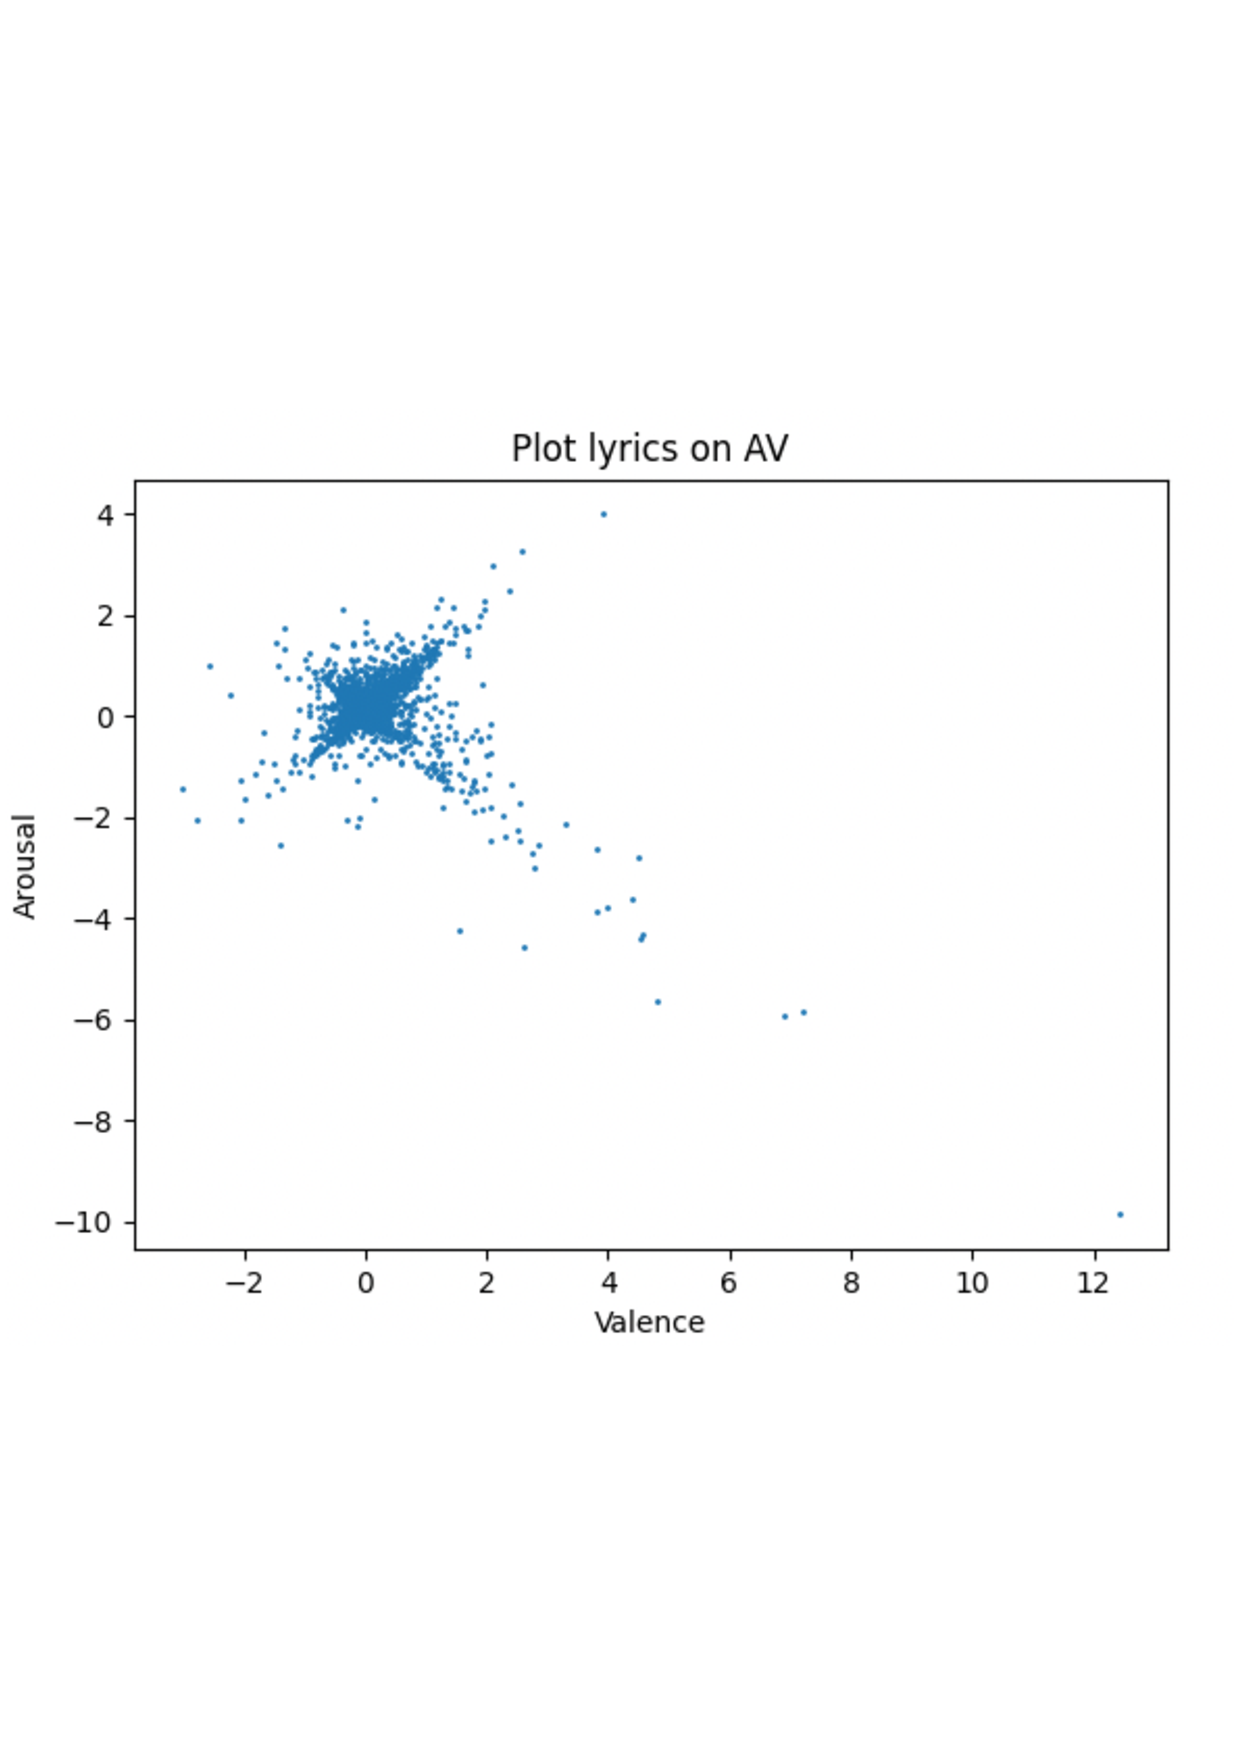
\includegraphics[width=12cm]{lyrics_AV.pdf}
    \vspace{0mm}
    \caption{歌詞 AV平面}
    \label{fig:vkall}
    \vspace{5mm}
\end{figure}

各印象ごとに歌詞を分類して,ward法で原点からの距離に基づいて3グループにクラスタリングした.
薄い肌色でプロットされている原点から一番近いグループを第1グループ.赤紫色でプロットされている原点から2番目に近いグループを第2グループ.黒色でプロットされている原点からもっとも遠いグループを第3グループとする.
\newpage
第1象限のプロット図は図3.3である.
\begin{figure}[H]
  \centering
  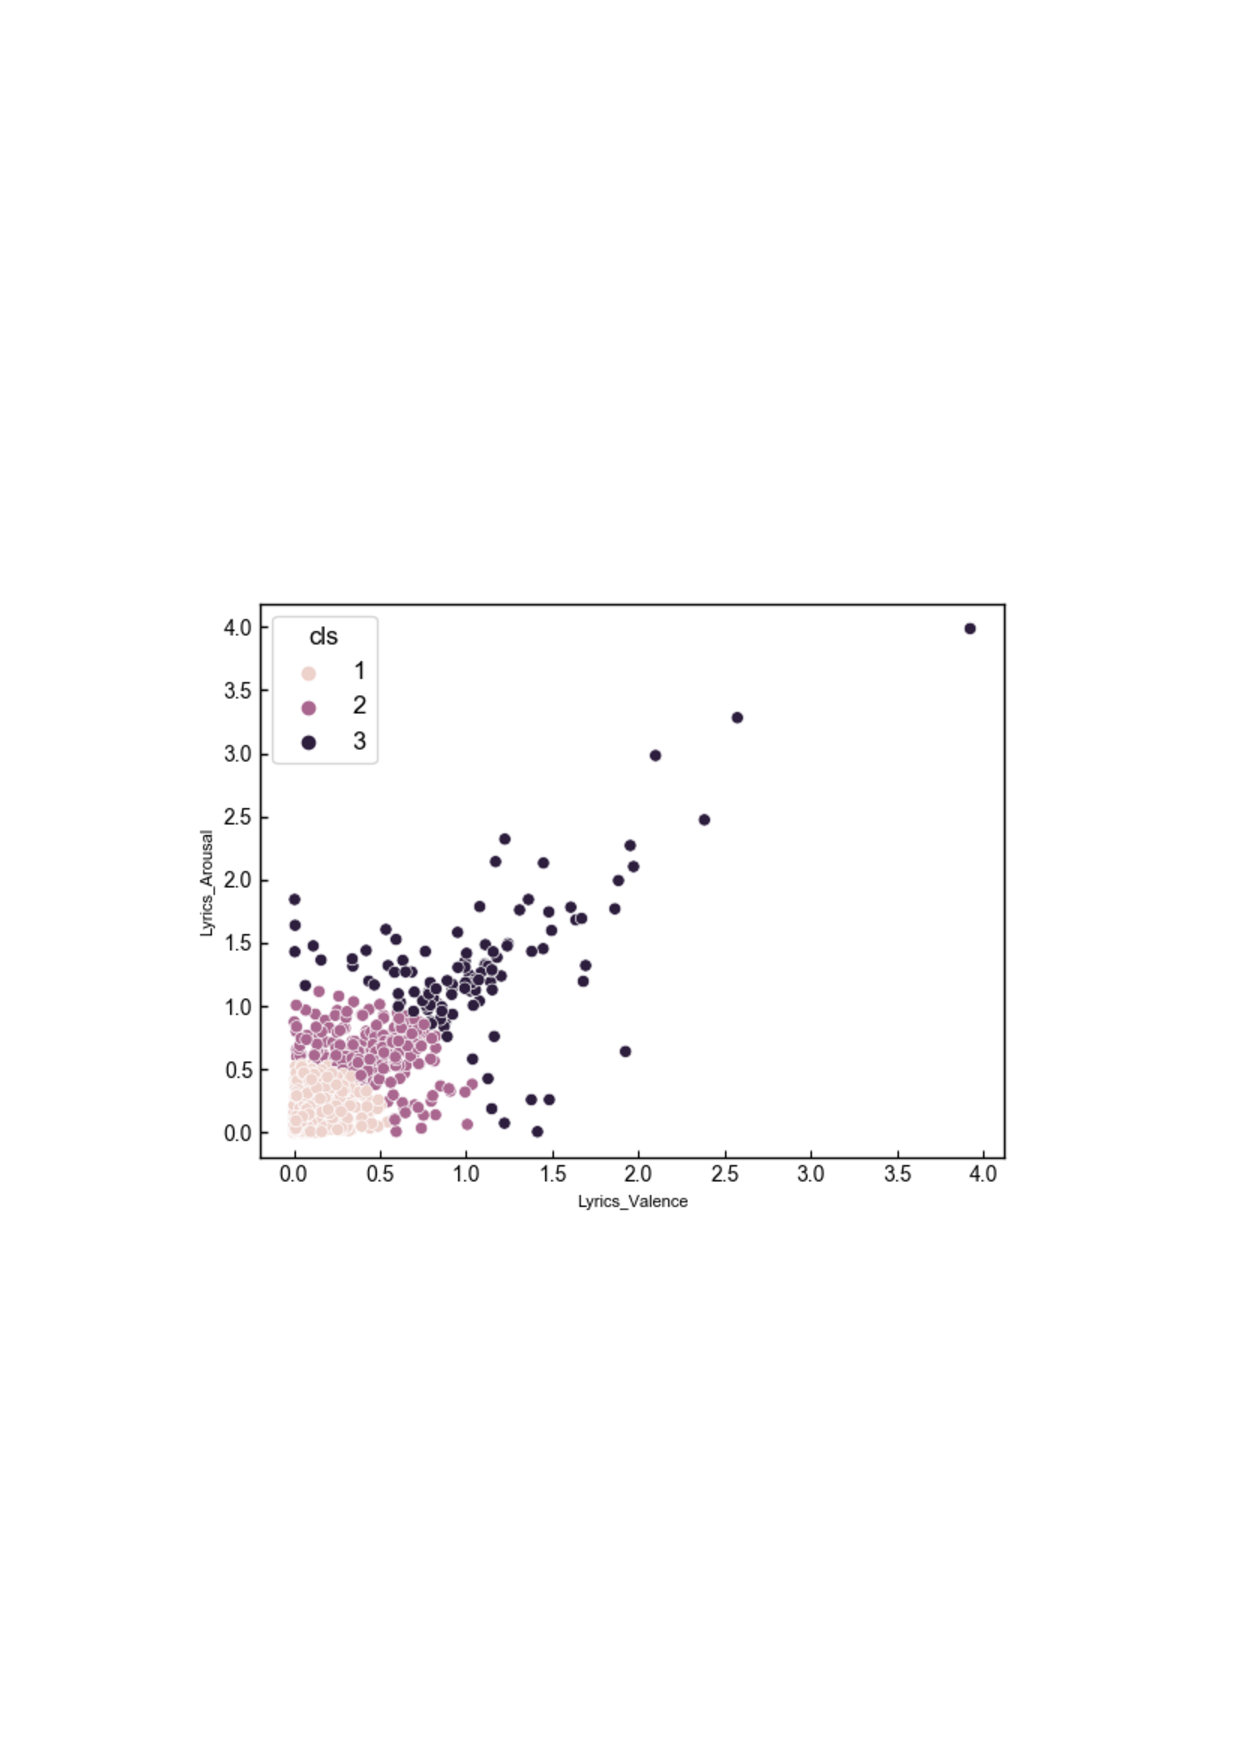
\includegraphics[width=14cm]{lyrics_A+V+.pdf}
  \vspace{-1mm}
  \caption{歌詞 A+V+平面}
  \label{fig:vkall}
  \vspace{5mm}
\end{figure}
第1象限にプロットされた楽曲は全部で1,424曲である.そのうちウォード法によって分割された曲数は第1グループが1015曲,第2グループが296曲,第3グループが112曲であった.
後述する実験に用いる楽曲の歌詞データはそれぞれのグループからランダムで1曲分選出する.
第1グループからはコブクロの「光の誓いが聴こえた日」,第2グループからは椎名林檎の「積み木遊び」,第3グループからはDREAM COME TRUEの「冬三昧にはまだ遠い」の3曲を選出した.
\newpage
第2象限のプロット図は図3.4である.
\begin{figure}[H]
  \centering
  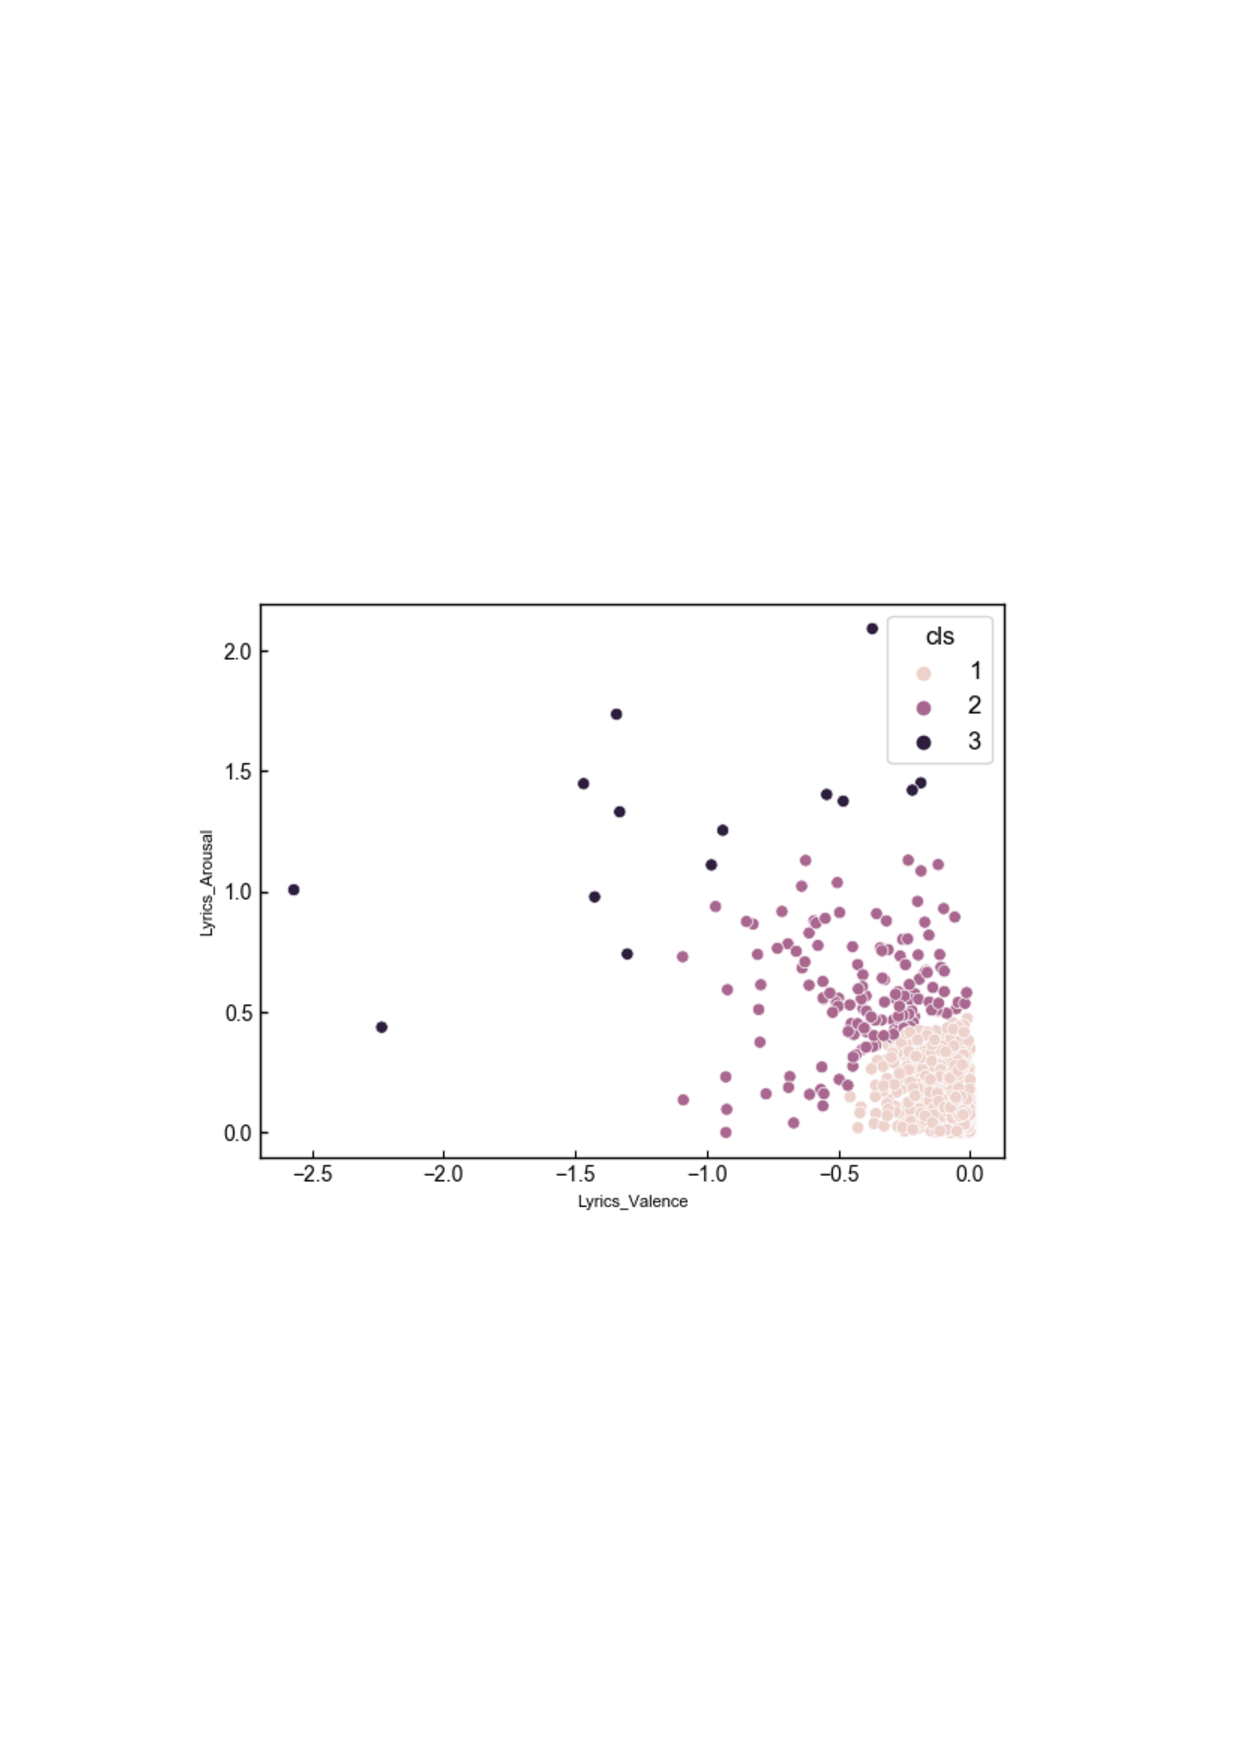
\includegraphics[width=14cm]{lyrics_A+V-.pdf}
  \vspace{-1mm}
  \caption{歌詞 A+V-平面}
  \label{fig:vkall}
  \vspace{5mm}
\end{figure}
第2象限にプロットされた楽曲は全部で887曲である.そのうちウォード法によって分割された曲数は第1グループが728曲,第2グループが145曲,第3グループが14曲であった.
後述する実験に用いる楽曲の歌詞データはそれぞれのグループからランダムで1曲分選出する.
第1グループからは,第2グループからはRADWIMPSの「透明人間18号」,第3グループからはB'zの「Da La Da Da」の3曲を選出した.
\newpage
第3象限のプロット図は図3.5である.
\begin{figure}[H]
  \centering
  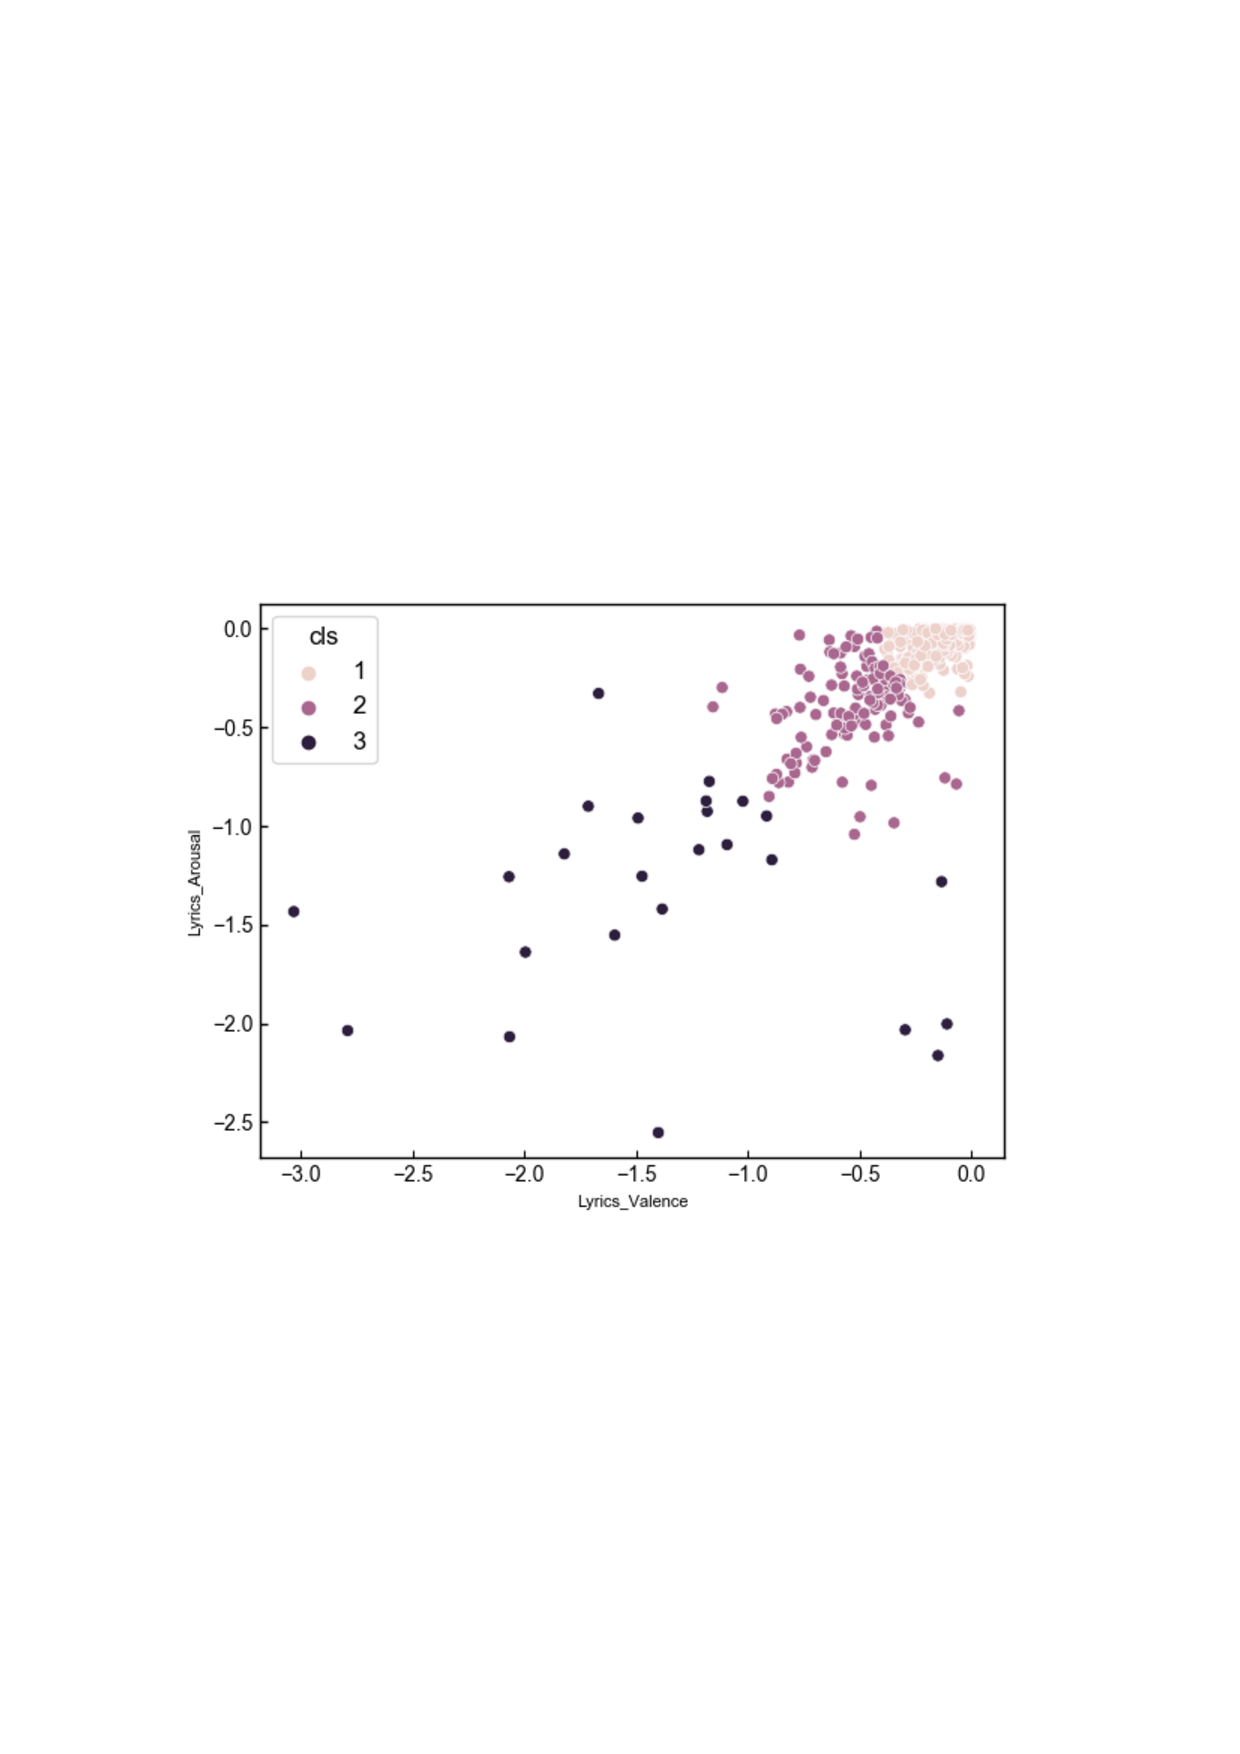
\includegraphics[width=14cm]{lyrics_A-V-.pdf}
  \vspace{-1mm}
  \caption{歌詞 A-V-平面}
  \label{fig:vkall}
  \vspace{5mm}
\end{figure}
第3象限にプロットされた楽曲は全部で388曲である.そのうちウォード法によって分割された曲数は第1グループが236曲,第2グループが127曲,第3グループが25曲であった.
後述する実験に用いる楽曲の歌詞データはそれぞれのグループからランダムで1曲分選出する.
第1グループからはEvery Little Thingの「Just be you」,第2グループからはコブクロの「コイン」,第3グループからはBUMP OF CHICKENの「分別奮闘記」の3曲を選出した.
\newpage
第4象限のプロット図は図3.6である.
\begin{figure}[H]
  \centering
  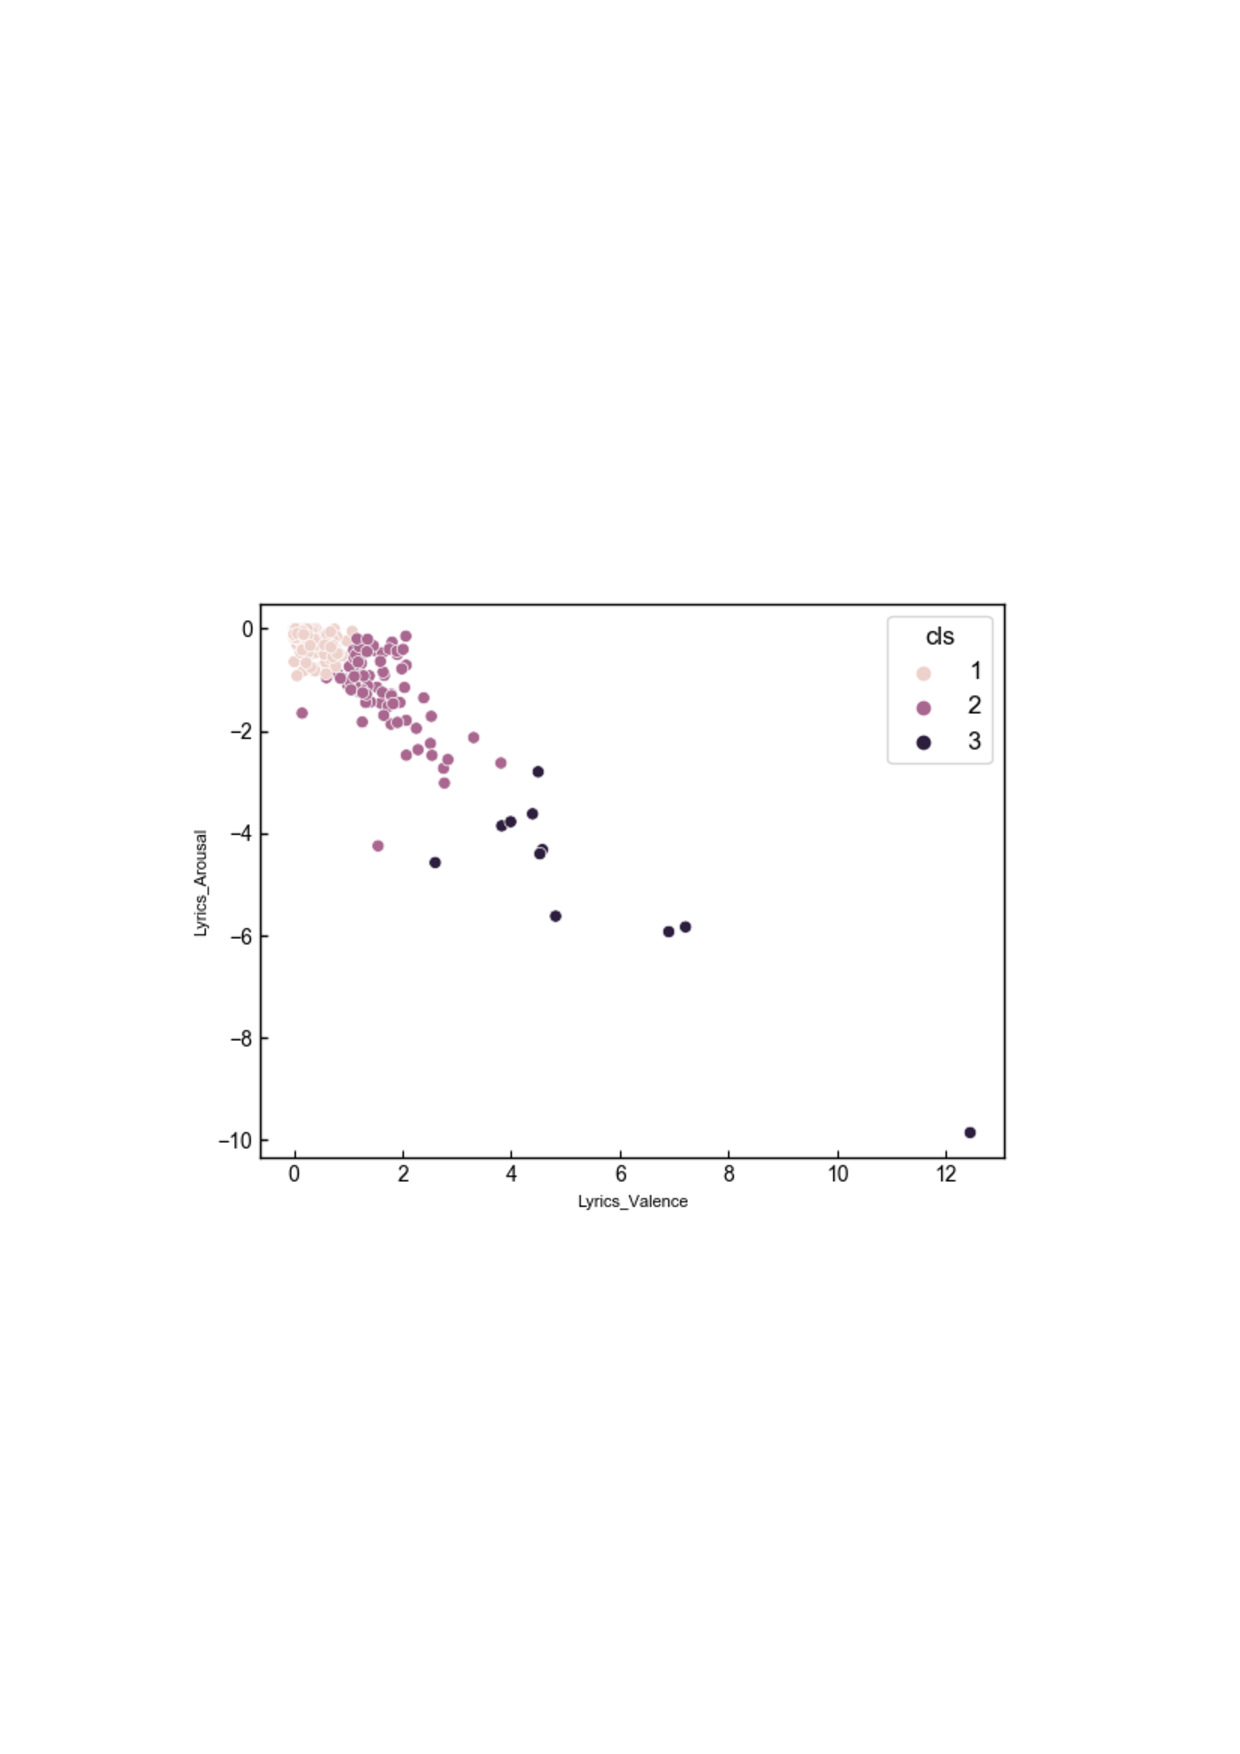
\includegraphics[width=14cm]{lyrics_A-V+.pdf}
  \vspace{-1mm}
  \caption{歌詞 A-V+平面}
  \label{fig:vkall}
  \vspace{5mm}
\end{figure}
第4象限にプロットされた楽曲は全部で302曲である.そのうちウォード法によって分割された曲数は第1グループが210曲,第2グループが81曲,第3グループが11曲であった.
後述する実験に用いる楽曲の歌詞データはそれぞれのグループからランダムで1曲分選出する.
第1グループからはUVERworldの「若さ故エンテレケイア」,第2グループからはあいみょんの「お互い様やん」,第3グループからはスピッツの「シロクマ」の3曲を選出した.
\newpage
\subsection{フレーズ}
歌詞に登場するフレーズをAV平面にプロットした.図3.7はAV平面に楽曲をプロットした図である.
\begin{figure}[H]
    \centering
    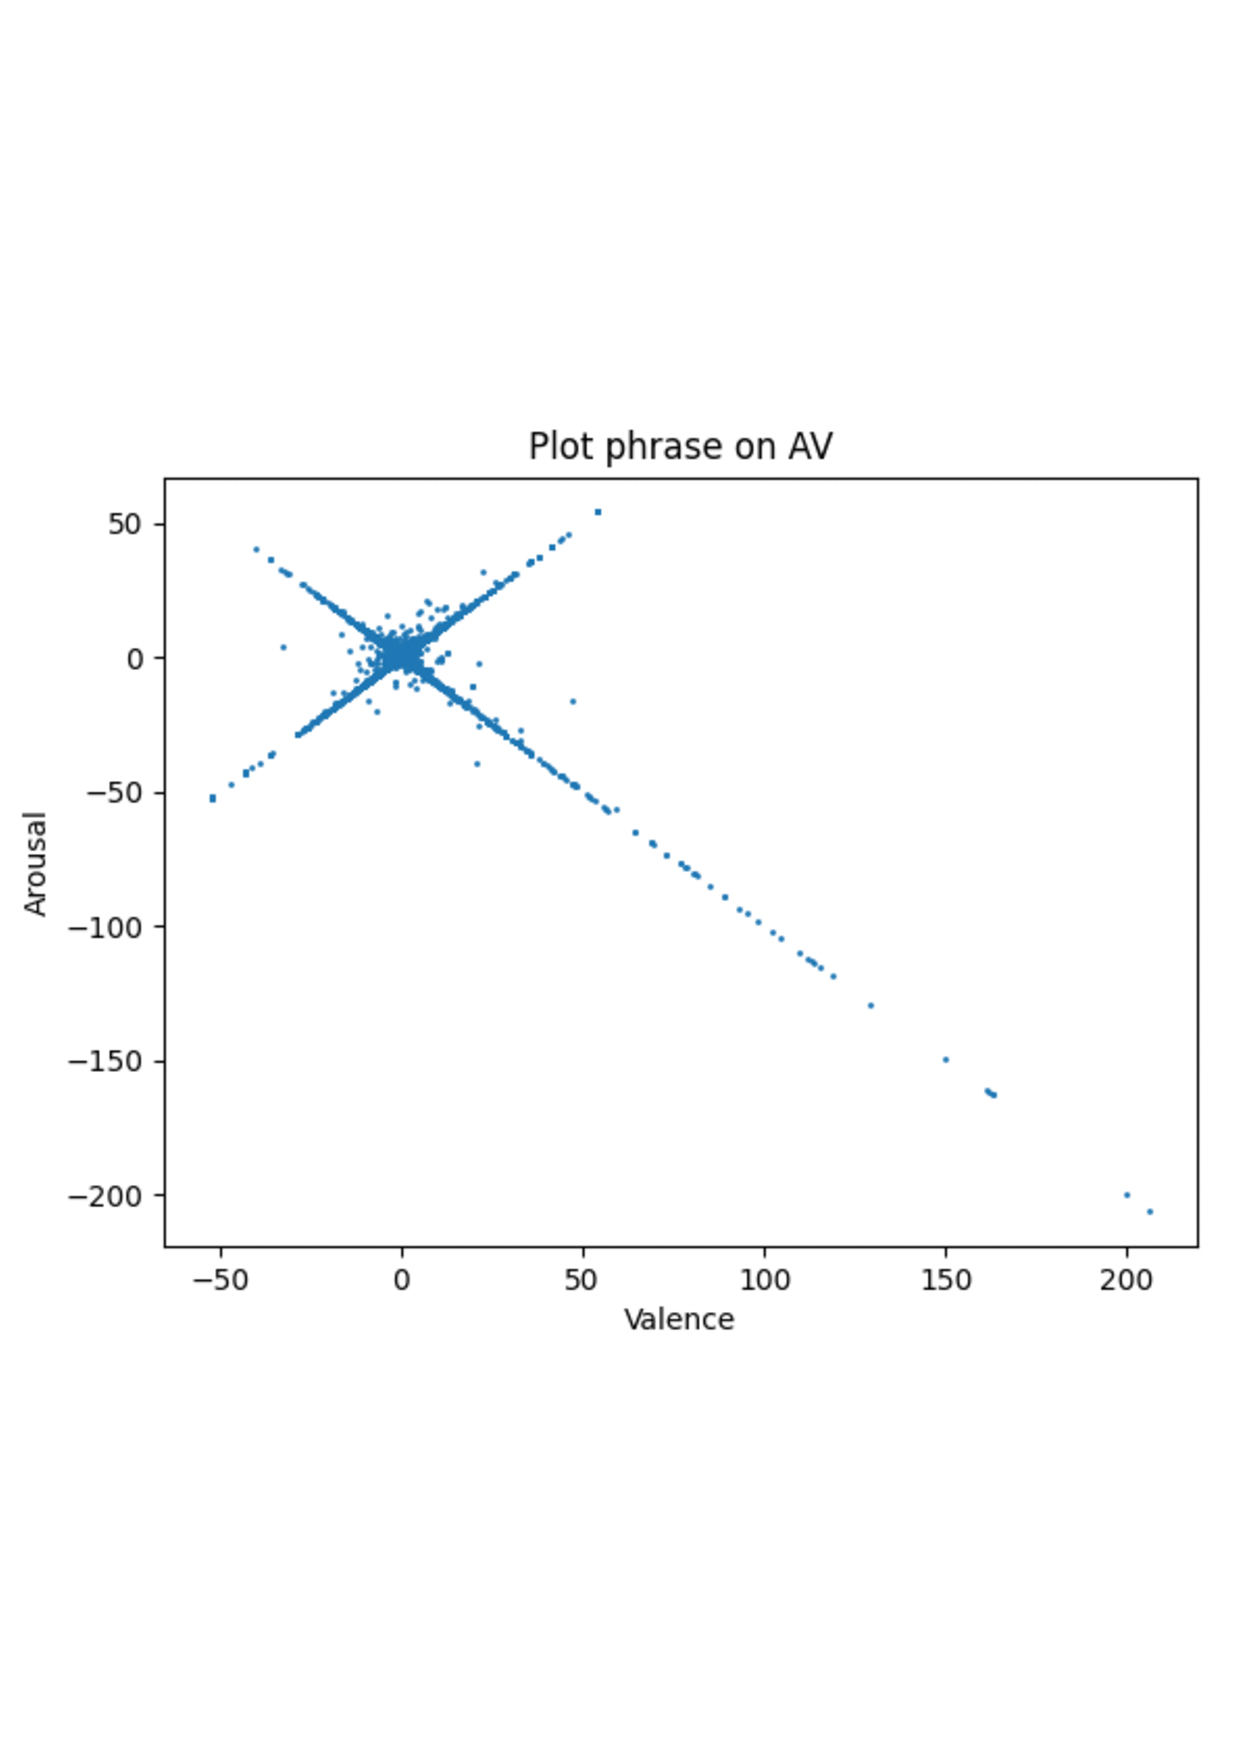
\includegraphics[width=12cm]{phrase_AV.pdf}
    \vspace{0mm}
    \caption{フレーズ AV平面}
    \label{fig:mms}
    \vspace{5mm}
\end{figure}
歌詞と同じく各印象ごとにフレーズを分類して,原点からの距離に基づいてward法でクラスタリングした.
\newpage
第1象限のプロット図は図3.8である
\begin{figure}[H]
    \centering
    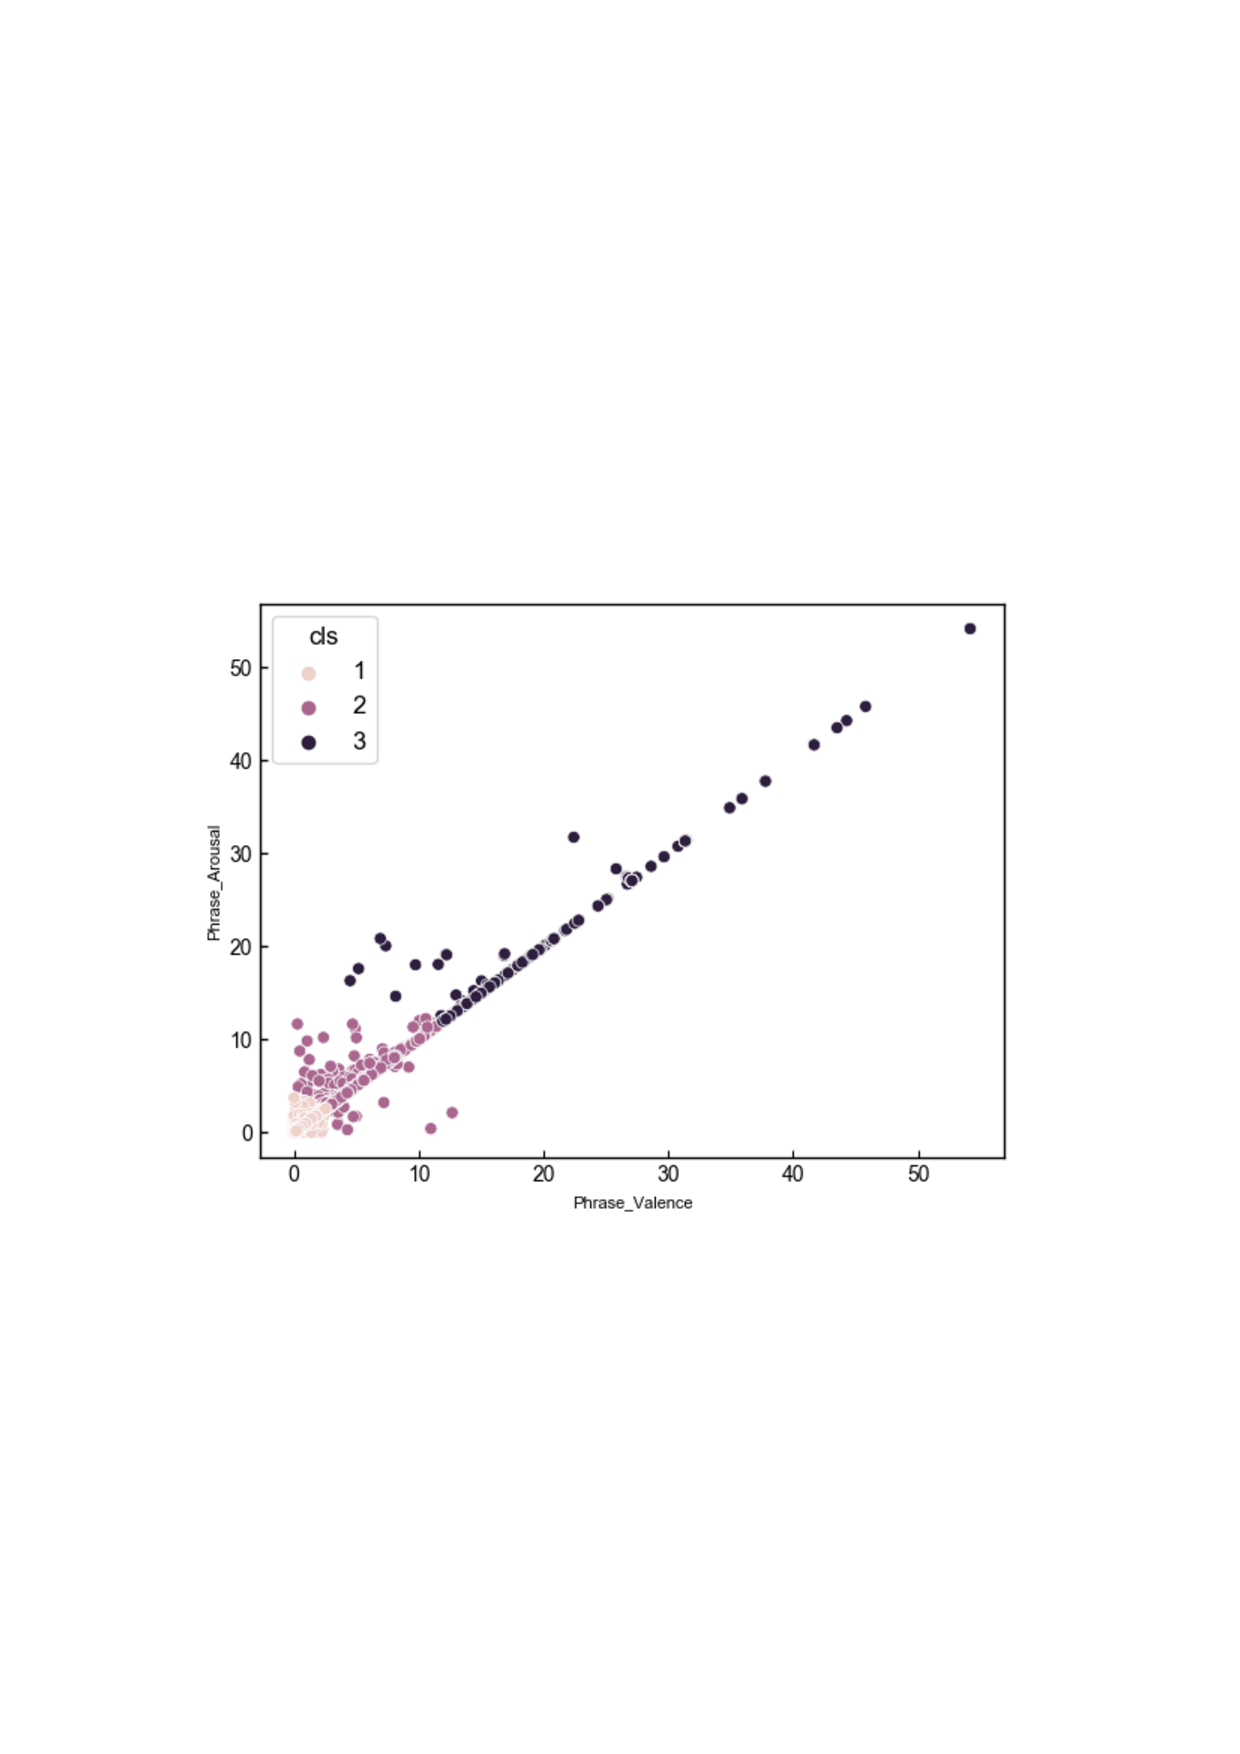
\includegraphics[width=14cm]{phrase_A+V+.pdf}
    \vspace{-1mm}
    \caption{フレーズ A+V+平面}
    \label{fig:mms}
    \vspace{5mm}
\end{figure}
第1象限にプロットされたフレーズは全部で35935句である.そのうちウォード法によって分割されたフレーズは第1グループが33,357句,第2グループが2,180句,第3グループが398句であった.
後述する実験に用いるフレーズのデータはそれぞれのグループからランダムで1句選出する.
第1グループからは「ひとりひとり違う世界みていくんだ」,第2グループからは「一石投じる生きる力」,第3グループからは「バタフライして」の3句を選出した.
\newpage
第2象限のプロット図は図3.9である.
\begin{figure}[H]
    \centering
    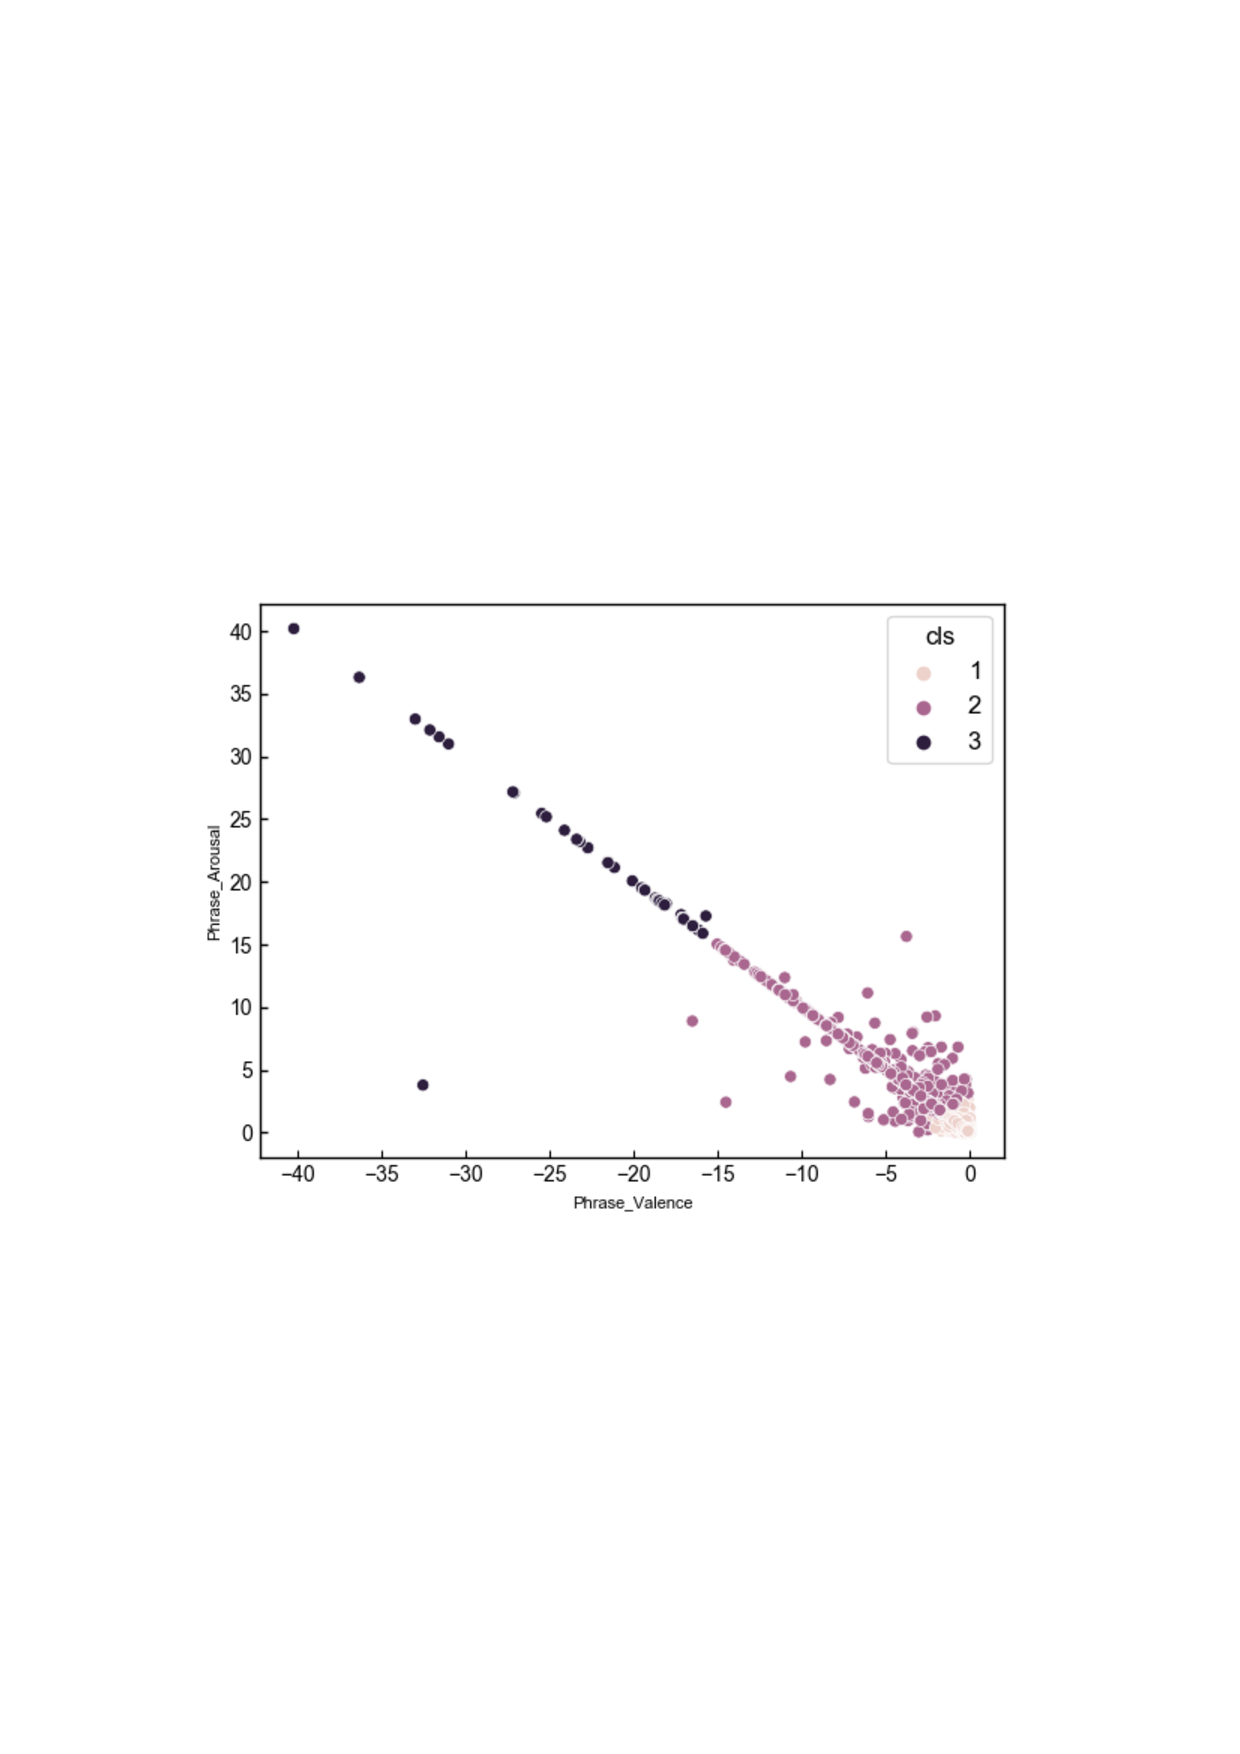
\includegraphics[width=14cm]{phrase_A+V-.pdf}
    \vspace{-1mm}
    \caption{フレーズ A+V-平面}
    \label{fig:mms}
    \vspace{5mm}
\end{figure}
第2象限にプロットされたフレーズは全部で27658句である.そのうちウォード法によって分割されたフレーズは第1グループが25,797句,第2グループが1,779句,第3グループが82句であった.
後述する実験に用いるフレーズのデータはそれぞれのグループからランダムで1句選出する.
第1グループからは「演じる意味はどこもブレたまま」,第2グループからは椎名林檎の「二つ並んだ影法師の手」,第3グループからはDREAM COME TRUEの「マイクホン争奪戦」の3句を選出した.
\newpage
第3象限のプロット図は図3.10である.
\begin{figure}[H]
    \centering
    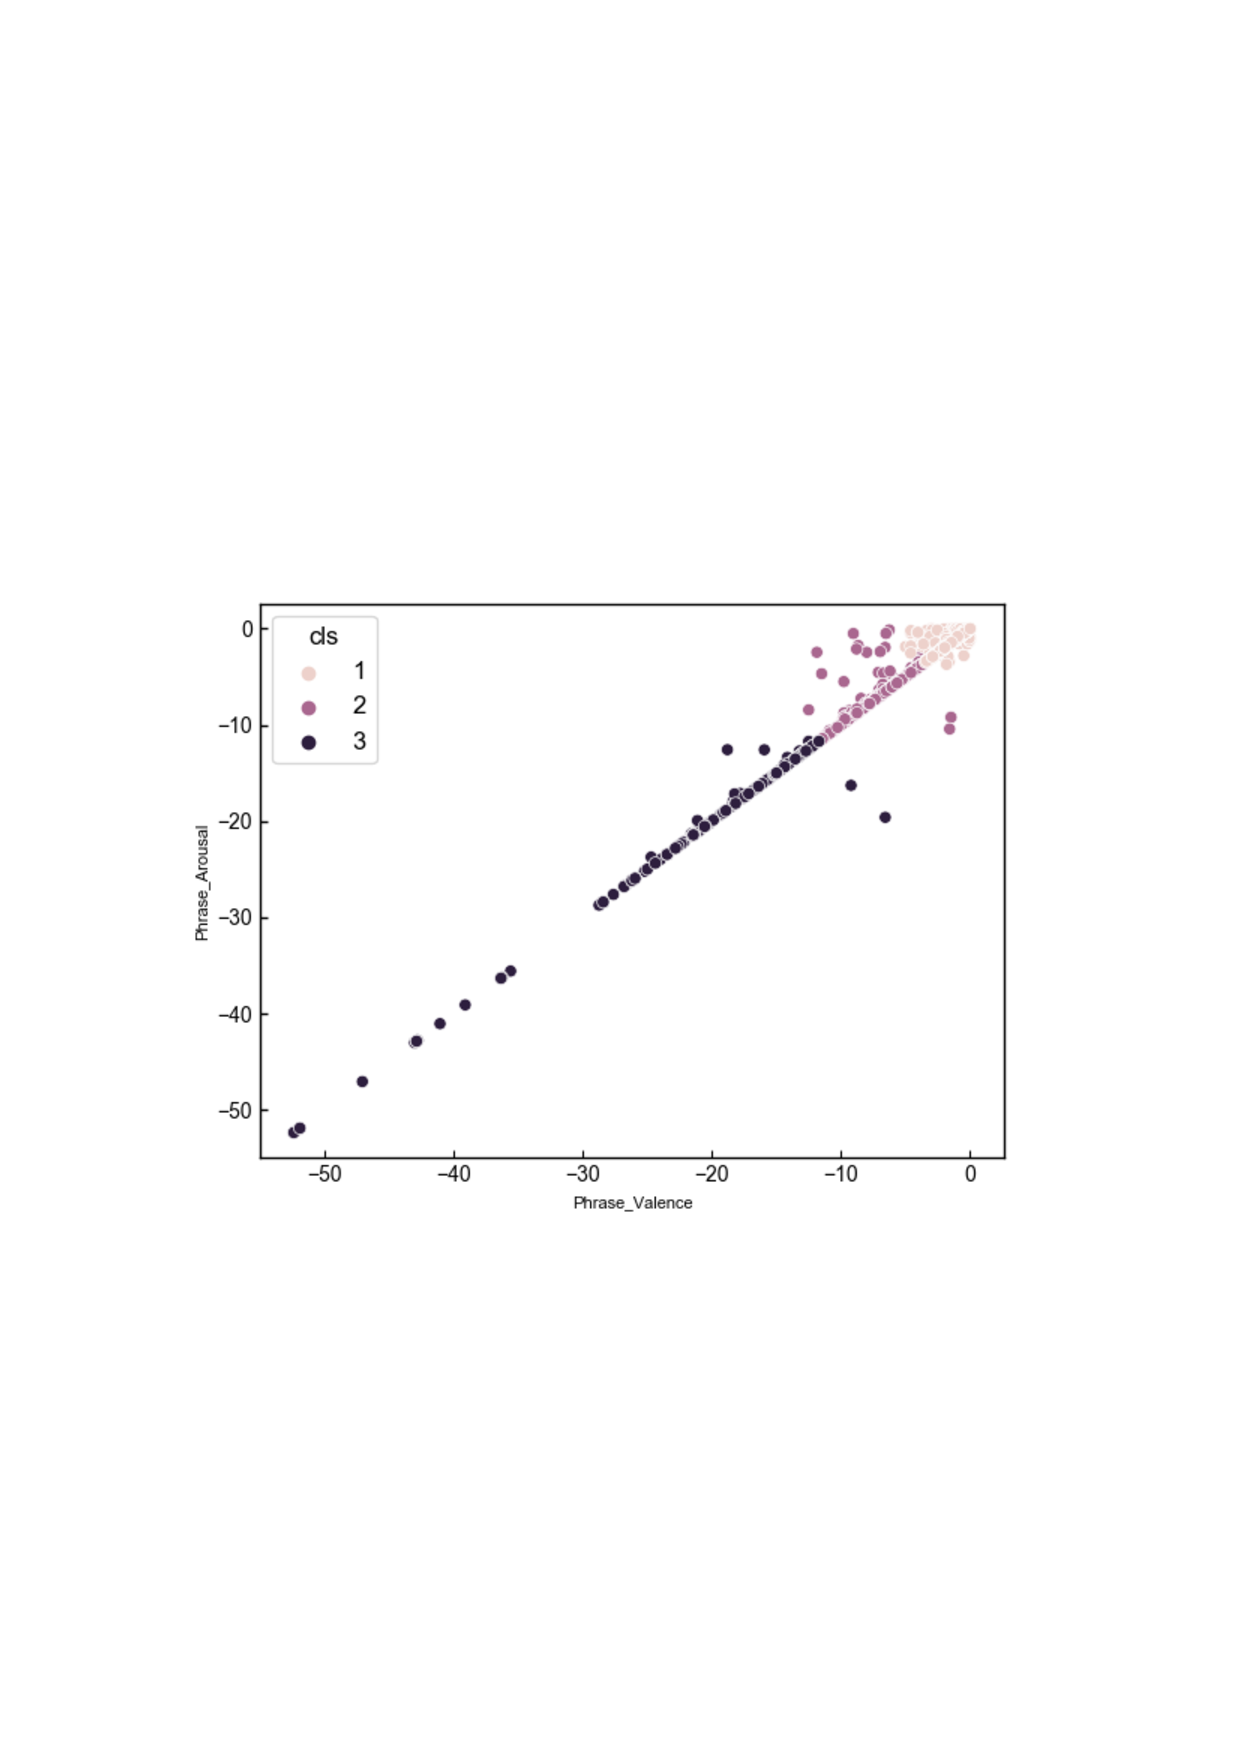
\includegraphics[width=14cm]{phrase_A-V-.pdf}
    \vspace{-1mm}
    \caption{フレーズ A-V-平面}
    \label{fig:mms}
    \vspace{5mm}
\end{figure}
第3象限にプロットされたフレーズは全部で14737句である.そのうちウォード法によって分割されたフレーズは第1グループが13,821句,第2グループが694句,第3グループが222句であった.
後述する実験に用いるフレーズのデータはそれぞれのグループからランダムで1句選出する.
第1グループからは「あたしを捨てたあなたは馬鹿で」,第2グループからは「あなたを苦しめたことでしょう」,第3グループからは「昨今のあなたは鼻につくわ」の3句を選出した.
\newpage
第4象限のプロット図は図3.11である.
\begin{figure}[H]
    \centering
    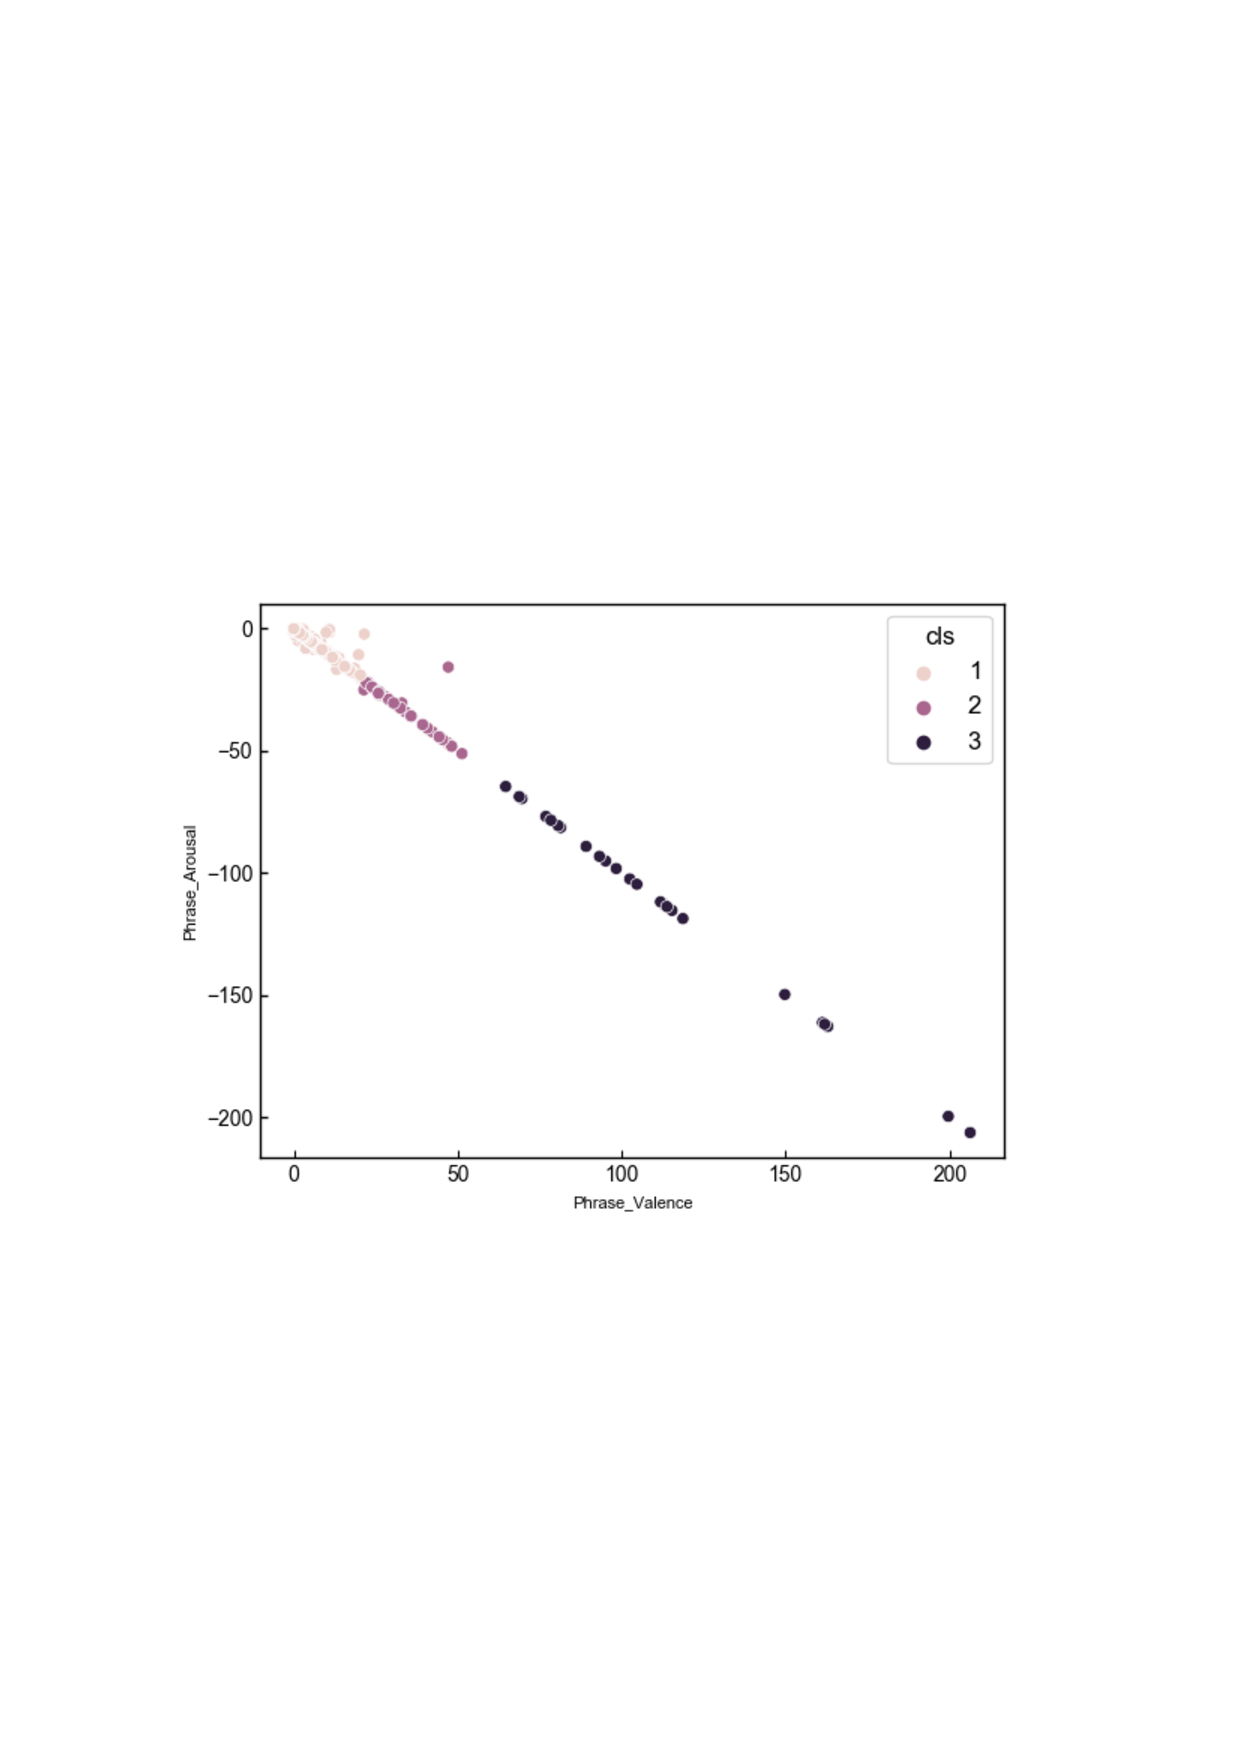
\includegraphics[width=14cm]{phrase_A-V+.pdf}
    \vspace{-1mm}
    \caption{フレーズ A-V+平面}
    \label{fig:mms}
    \vspace{5mm}
\end{figure}
第4象限にプロットされたフレーズは全部で60,000句以上である.第4象限にプロットされたフレーズ数は多かったので,重複削除をした後にランダムで30,000句を取り出した.そのうちウォード法によって分割されたフレーズは第1グループが29,907句,第2グループが64句,第3グループが29句であった.
後述する実験に用いるフレーズのデータはそれぞれのグループからランダムで1句選出する.
第1グループからは「浮かぶ月にやさしく響いては消えてった」,第2グループからは「染まる真っ赤なギロチン」,第3グループからは「しぶといトラウマも全部払おう」の3句を選出した.

%
\end{document} % 3章
\documentclass[a4paper,11pt,oneside,openany]{jsbook}
\usepackage{myjlabthesisstyle}
\daigaku{青山学院大学}
\gakubu{社会情報学部}
\gakka{社会情報学科}
\syubetsu{卒業論文}
\labname{宮治研究室}
\chiefexaminer{宮治~~裕~~教授}

%%%%%%%%%%%%%%%%%%%%%%%%%%%%%%%%%%%%%%%
% ここから先「ここまで個人設定」の範囲に
% 各自の固有の情報を記入して下さい
%%%%%%%%%%%%%%%%%%%%%%%%%%%%%%%%%%%%%%%
\nendo{2021年度}
\teisyutsu{2022年~~1月}
\snum{18118047}
\jname{黒川~~皇輝}
\thesistitle{PLSAとMAP推定を用いた日本語歌詞の印象推定手法の評価} %タイトルを記入
%\thesissubtitle{\LaTeX の利用} %サブタイトルを記入 ない場合はコメントアウト
%\SUBTtrue %サブタイトル有りの場合 ない場合は,コメントアウト
\SUBTfalse %サブタイトル無しの場合 有る場合は,コメントアウト
%%%%%%%%%% ここまで個人設定 %%%%%%%%%%%%%%
\begin{document}

\chapter{Visual Studio Codeで編集する人へ}
Visual Studio Codeを使って \LaTeX 論文を作成する人が増えているため、それに合わせた修正を各所でおこなっている。
以下の設定や、注意事項を参照してほしい。

\section{コンパイルのための設定}
\LaTeX をコンパイルする際には、目次や参照、参考文献などを組み込むための処理などを複数回実行する必要がある。
これを自動で判断して実行するための設定ファイルが \verb+.latexmkrc+である。
本スタイルファイルパッケージでは、以下の設定をしている。
\begin{screen}
{\small
\begin{verbatim}
#!/usr/bin/env perl
$pdf_mode = 3;
$latex = 'platex -halt-on-error';
$bibtex = 'pbibtex';
$dvipdf = 'dvipdfmx %O -o %D %S';
\end{verbatim}    
}
\end{screen}

なお、一部の行を割愛して表示している。
詳細は、直接ファイルを確認してほしい。

情報源として、以下の2サイトを記載する。
Macintosh だけでなく、WindowsやLinuxでの利用(特にプレビュー)を含めた設定については、\verb+@popunbom+氏のQiitaの記事「VSCode で LaTeX を書く (2018)」~\cite{popunbom1}が詳しい。
LaTeXをインストールしたり、利用したりする際の情報源である \TeX Wiki にも「Visual Studio Code/LaTeX」~\cite{texwikivscode}なるページがある。

\section{LaTeX Workshop の設定}
VSCodeプラグインであるLaTeX Workshopの設定は、以下の様にしている。
なお、必ずしも同じ設定にする必要はない。
\begin{screen}
{\footnotesize
\begin{verbatim}
"latex-workshop.latex.tools": [
  {
    "name": "Latexmk (pLaTeX)",
    "command": "latexmk",
    "args": [
      "-f",
      "-gg",
      "-pv",
      "-latex='platex'",
      "-synctex=1",
      "-interaction=nonstopmode",
      "-file-line-error",
      "%DOC%"
    ]
  },
],
\end{verbatim}
}
\end{screen}
\begin{screen}
    {\footnotesize
    \begin{verbatim}
"latex-workshop.latex.recipes": [
  {
    "name": "pLaTeX",
    "tools": [
      "Latexmk (pLaTeX)"
    ]
  },
],
\end{verbatim}
}
\end{screen}
\begin{screen}
{\footnotesize
\begin{verbatim}
"latex-workshop.latex.magic.args": [
  "-f",
  "-gg",
  "-pv",
  "-synctex=1",
  "-interaction=nonstopmode",
  "-file-line-error",
  "%DOC%"
],
\end{verbatim}
}
\end{screen}
\begin{screen}
{\footnotesize
\begin{verbatim}
"latex-workshop.view.pdf.viewer":"tab",
"latex-workshop.latex.autoBuild.run": "never",
"latex-workshop.view.pdf.refviewer":"tabOrBrowser",
"latex-workshop.latex.autoClean.run":"onBuilt",
\end{verbatim}
}
\end{screen}

\section{分割(子ファイル)コンパイル}
通常の \LaTeX のファイルの場合に親ファイルに記述する文書開始や終了/スタイルファイルの読み込みを子ファイル側に書き込むことによって、それぞれのファイルごとにコンパイルができる。

\begin{screen}
{\footnotesize
\begin{verbatim}
\documentclass[a4paper,10pt,twocolumn]{jsarticle}
\usepackage{myjlababsstyle}
\begin{document}
\section{これは読み込まれる子ファイルの例}
ファイル名は sub.tex とします。
\end{document}
\end{verbatim}
}
\end{screen}

これを読み込む親ファイル側では、これらの設定を無視するようにしなければならない。
そのために、\verb+docmute+パッケージを用いている。
親ファイルの例を以下に示す。
\begin{screen}
{\footnotesize
\begin{verbatim}
\documentclass[a4paper,10pt,twocolumn]{jsarticle}
\usepackage{docmute}
\usepackage{myjlababsstyle}
\begin{document}
これは親ファイルの例です。
\input{sub}
\end{document}
\end{verbatim}
}
\end{screen}

また、多くのスタイルファイルを親ファイルと子ファイルで共通して読み込むために、スタイルファイルを \verb+myjlababsstyle.sty+ ファイル内に列挙している。
各自でスタイルファイルを追加する場合には、このファイルに記載すること。

\section{テキスト校正くん}
「テキスト校正くん」パッケージは追加すべきである。
ただし、\LaTeX のファイルは校正してくれないため、\verb+txt+か\verb+md+のファイルを作成し、そこに文章を貼り付けて校正するのが良い。
インストールや設定などが必要ない「テキスト校正くん」を利用することにしたが、昨年まではRedpenと比較して細かい部分の校正は不十分である。
最低限の校正として必ず利用してほしい。
%
\end{document}
 % 4章
\documentclass[a4paper,11pt,oneside,openany]{jsbook}
\usepackage{myjlabthesisstyle}
\daigaku{青山学院大学}
\gakubu{社会情報学部}
\gakka{社会情報学科}
\syubetsu{卒業論文}
\labname{宮治研究室}
\chiefexaminer{宮治~~裕~~教授}

%%%%%%%%%%%%%%%%%%%%%%%%%%%%%%%%%%%%%%%
% ここから先「ここまで個人設定」の範囲に
% 各自の固有の情報を記入して下さい
%%%%%%%%%%%%%%%%%%%%%%%%%%%%%%%%%%%%%%%
\nendo{2021年度}
\teisyutsu{2022年~~1月}
\snum{18118047}
\jname{黒川~~皇輝}
\thesistitle{PLSAとMAP推定を用いた日本語歌詞の印象推定手法の評価} %タイトルを記入
%\thesissubtitle{\LaTeX の利用} %サブタイトルを記入 ない場合はコメントアウト
%\SUBTtrue %サブタイトル有りの場合 ない場合は,コメントアウト
\SUBTfalse %サブタイトル無しの場合 有る場合は,コメントアウト
%%%%%%%%%% ここまで個人設定 %%%%%%%%%%%%%%
\begin{document}

\chapter{おわりに}
本章では本研究のまとめと今後の課題について述べる.
\section{まとめ}
本研究ではコンテキストアウェア楽曲推薦システムの今後の発展のために日本語歌詞の印象推定手法の設計と効果測定をおこなった.
従来の歌詞の印象推定手法は未だ発展途上にあり,詳細に印象推定できる手法は未だ存在しない.そのため西川らの設計した印象推定手法に基づき日本語歌詞の印象推定方法を設計した.
4章で述べた実験結果より設計した印象推定手法は一部の印象において妥当であることが判明した.しかし,全体的には印象を推定することは叶わなかったと言える.
一部の印象を推定できた理由としては事前知識が十分に存在したことが考えられる.
\section{今後の課題}
今後の課題は2点ある.1つ目は事前知識を増やす必要があることである.日本語版ANEW拡張データセットは印象においてデータ数に偏りが認められ,印象推定の結果が妥当であると判断された印象の事前知識は不当であると判断された印象よりも2,000語多く存在した.
したがって推定結果が不当であった印象における事前知識を増やす必要があると考える.
2つ目は歌詞から得られる印象が必ずしも1つではないということを考慮する必要があることである.歌詞全体の印象はフレーズから得られる印象の合計値であると本研究では推測して実験をおこなった.
しかし,歌詞によっては複数の印象を与える歌詞も存在するため,必ずしも1つの印象に推定することは正しいと言えない.そのため,複数の印象を推定するという観点で推定手法を設計し直す必要がある.
\end{document} % 5章
%\include{chap6} % 6章
%\include{chap7} % 7章
\end{verbatim}
}
\end{breakbox}

なお、これらのファイルは通常の\verb+\chapter+など \LaTeX の命令でマークアップしていけば良い。
chapter1.tex や chapter2.tex、chapter3.tex 内を見れば、おおよその方法は理解できるはずである。

\subsection{付録の設定と読み込み}
付録は以下の様になっている。
\begin{breakbox}
{\small
%footnotesize
\begin{verbatim}
%%% 付録 -- 必要なければ以下を2行コメントアウト
\appendix
\documentclass[a4paper,11pt,oneside,openany]{jsbook}
\usepackage{myjlabthesisstyle}
\daigaku{青山学院大学}
\gakubu{社会情報学部}
\gakka{社会情報学科}
\syubetsu{卒業論文}
\labname{宮治研究室}
\chiefexaminer{宮治~~裕~~教授}

%%%%%%%%%%%%%%%%%%%%%%%%%%%%%%%%%%%%%%%
% ここから先「ここまで個人設定」の範囲に
% 各自の固有の情報を記入して下さい
%%%%%%%%%%%%%%%%%%%%%%%%%%%%%%%%%%%%%%%
\nendo{2021年度}
\teisyutsu{2022年~~1月}
\snum{18118047}
\jname{黒川~~皇輝}
\thesistitle{PLSAとMAP推定を用いた日本語歌詞の印象推定手法の評価} %タイトルを記入
%\thesissubtitle{\LaTeX の利用} %サブタイトルを記入 ない場合はコメントアウト
%\SUBTtrue %サブタイトル有りの場合 ない場合は,コメントアウト
\SUBTfalse %サブタイトル無しの場合 有る場合は,コメントアウト
%%%%%%%%%% ここまで個人設定 %%%%%%%%%%%%%%
\begin{document}

\chapter{プログラムの動作方法}
本研究にて用いたプログラムについて解説する。

\section{ファイル構成}
プログラムのフォルダ内は、主に4つのファイルから構成される。

ああああいいいい

ううううええええ

これらを○○に設置し、以下の手順にそって起動する。

\section{起動方法}
まず、ウェブサーバを動かした状態にし、外部クライアント(Webブラウザから)、以下のURLにアクセスする。


\section{表示の見方}
実験に利用するための、実行結果は test.log ファイルに出力されている。

このファイルは4つのカラムからなる CSV形式のファイルである。
第1列には、…

%
\end{document}




%\include{appendixB} %必要に応じて付録の数を増やす
\end{verbatim}
}
\end{breakbox}
サンプルとして 付録A(appendixA.tex)だけ読み込む様にしている。
このファイルも通常の\verb+\chapter+など通常の\LaTeX の命令でマークアップしていけば良い。
また、必要に応じて追加、コメントアウトして構わない。

\subsection{参考文献の設定と読み込み}
最後に参考文献の設定がなされている。
\begin{breakbox}
{\small
%footnotesize
\begin{verbatim}
\bibliographystyle{junsrt}
\bibliography{myrefs}
\end{verbatim}
}
\end{breakbox}
\verb+\bibliography{myrefs}+によって myrefs.bib ファイルが読み込まれている。
このファイルは \BibTeX のフォーマットにて記載されている。
詳細は3章にて記述する。
